\section{Optik}

\subsection{Licht}

Licht kann auf mehrere Arten beschrieben werden:


\subsubsection{Lichtstrahlen}

\begin{minipage}{0.48\linewidth}
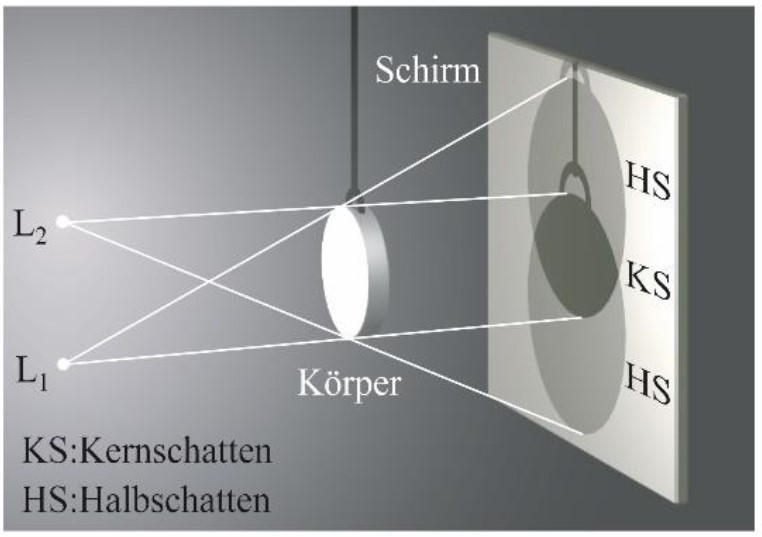
\includegraphics[width=\linewidth]{Bilder/Wellen-Optik/lichtstrahlen}
\end{minipage}
\hfill
\begin{minipage}{0.48\linewidth}
Die \textbf{geometrische Optik} oder \textbf{Strahlenoptik} geht davon aus, dass sich das Licht im Vakuum als \textbf{geradliniger Strahl} ausbreitet.\\
\\
Mit der geometrischen Optik können die Phänomene Reflexion und Brechung erklärt werden.
\end{minipage}



\subsubsection{Lichtwellen}


\begin{minipage}{0.48\linewidth}
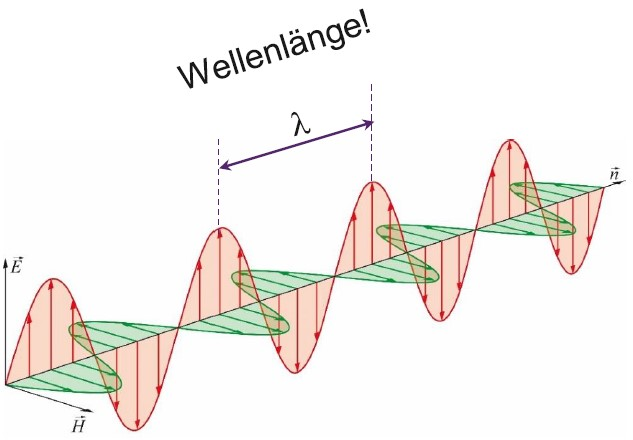
\includegraphics[width=\linewidth]{Bilder/Wellen-Optik/lichtwelle} \\
\\
\end{minipage}
\hfill
\begin{minipage}{0.48\linewidth}
Licht wird als elektromagnetische Welle modelliert.  \\
\\
Bild: linear polarisierte \\
Welle \\
\end{minipage}

\textbf{Lichtfarben und ihre Frequenzen / Wellenlängen} \\
\begin{minipage}{0.5\linewidth}
	\begin{tabular}{| l | c |}
		\hline
		\textbf{Farbe} & \textbf{Wellenlänge in $\mathrm{nm}$} \\
		\hline
		\color{red!50!blue!80!white}violett & 380 ... 435 \\
		\hline
		\color{blue}blau & 435 ... 465 \\
		\hline
		\color[HTML]{35c2bd}blaugrün & 465 ... 485 \\
		\hline
		\color{green!80!black}grün & 485 ... 565 \\
		\hline
		\color{yellow!75!red}gelb & 565 ... 590 \\
		\hline
		\color{orange}orange & 590 ... 630 \\
		\hline
		\color{red}rot & 630 ... 780 \\
		\hline
	\end{tabular}
\end{minipage}
	\hfill
\begin{minipage}{0.5\linewidth}
	\begin{center}
		$$ \boxed{ \lambda = \frac{c}{f} } $$

		$$ \boxed{ \frac{\Delta f}{\Delta \lambda} = -\frac{c}{\lambda^2} } $$
	\end{center}
\end{minipage}

\begin{tabular}{c l c}
	$\lambda$ & Wellenlänge & $[\lambda] = \m$ \\
	$c$ & Lichtgeschw. $c = 299'792'458 \mathrm{\frac{m}{s}}$ & $[c] = \mathrm{\frac{m}{s}}$ \\
	$f$ & Frequenz & $[f] = \mathrm{\frac{1}{s} = Hz}$ \\
\end{tabular}




\subsubsection{Lichtteilchen}

Modellvorstellung des Lichts als ein Fluss von Lichtteilchen (\textbf{Photonen}) \\


$$ \boxed{ E = h \cdot f } $$

\begin{tabular}{c l c}
	$E$ & Energie \textbf{eines} Photons & $[E] = \J$ \\
	$h$ & Planck'sche Konstante $6.626 \cdot 10^{-34} \frac{\J}{\Hz}$ & $[h] = \frac{\J}{\Hz}$ \\
	$f$ & Frequenz & $[f] = \mathrm{\frac{1}{s} = Hz}$ \\
\end{tabular}



\subsection{Lichtquellen}

\subsubsection{Thermische Strahler}

\textbf{Schwarzkörper-Modell}: Modell eines Körpers, der in alle \\
Richtungen abstrahlt (und energetisch im Gleichgewicht ist) \\
\\
Ein Schwarzkörper strahlt \textbf{alle} Lichtfarben ab. (auch die für den Mensch nicht sichtbaren.) \\
\\

\begin{minipage}{0.48\linewidth}
\textbf{Glühbirnen} \\
\\
Muss auf allen Wellenlängen angeregt werden, um schliesslich sichtbares Licht abzustrahlen. \\
$\Rightarrow$ Es wird viel Energie nicht nutzbar 'verheizt'
\end{minipage}
\hfill
\begin{minipage}{0.48\linewidth}
\textbf{LEDs} \\
\\
Können mit einer bestimmten Frequenz angeregt werden und strahlen nur gewünschtes Licht ab. \\
$\Rightarrow$ energieeffizient
\end{minipage}



\subsubsection{Lumineszenz}

\begin{minipage}{0.3\linewidth}
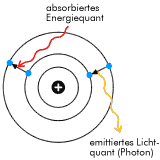
\includegraphics[width=\linewidth]{Bilder/Wellen-Optik/lumineszenz}
\end{minipage}
\hfill
\begin{minipage}{0.58\linewidth}
Elektronen werden angeregt und steigen in energetisch höheren Zustand. \\
Sobald die Elektronen wieder in ihren Grundzustand zurückkehren wird ein Lichtquant (Photon) abgestrahlt. \\
Die Leuchtfarbe wird durch die \\
Frequenz der Anregung bestimmt. \\
\\
\textbf{Fluoreszenz}: kein Nachleuchten \\
\textbf{Phosphoreszenz}: mit Nachleuchten \\
\end{minipage}

% \vfill\null
% \columnbreak



\subsection{Messgrössen}

\subsubsection{Radiometrie}
Physikalische Messgrössen der elekromagnetischen Strahlung


\subsubsection{Photometrie}
Radiometrische Grössen, gewichtet mit dem photometrischen Strahlungsäquivalent $K$, welches die \textbf{Empfindlichkeit des menschlichen Auges} angibt. \\
\\
\textbf{Photometrischen Strahlungsäquivalent $K$} \\
Gibt die Empfindlichkeit des menschlichen Auges wieder und ist eine empirisch genormte Kurve \\
$\Rightarrow$ Das menschliche Auge ist bei einer Wellenlänge von $555 \, \mathrm{nm}$ \\ (grüne Farbe) am empfindlichsten. (638 $\frac{lm}{W}$)




\subsection{Gegenüberstellung}

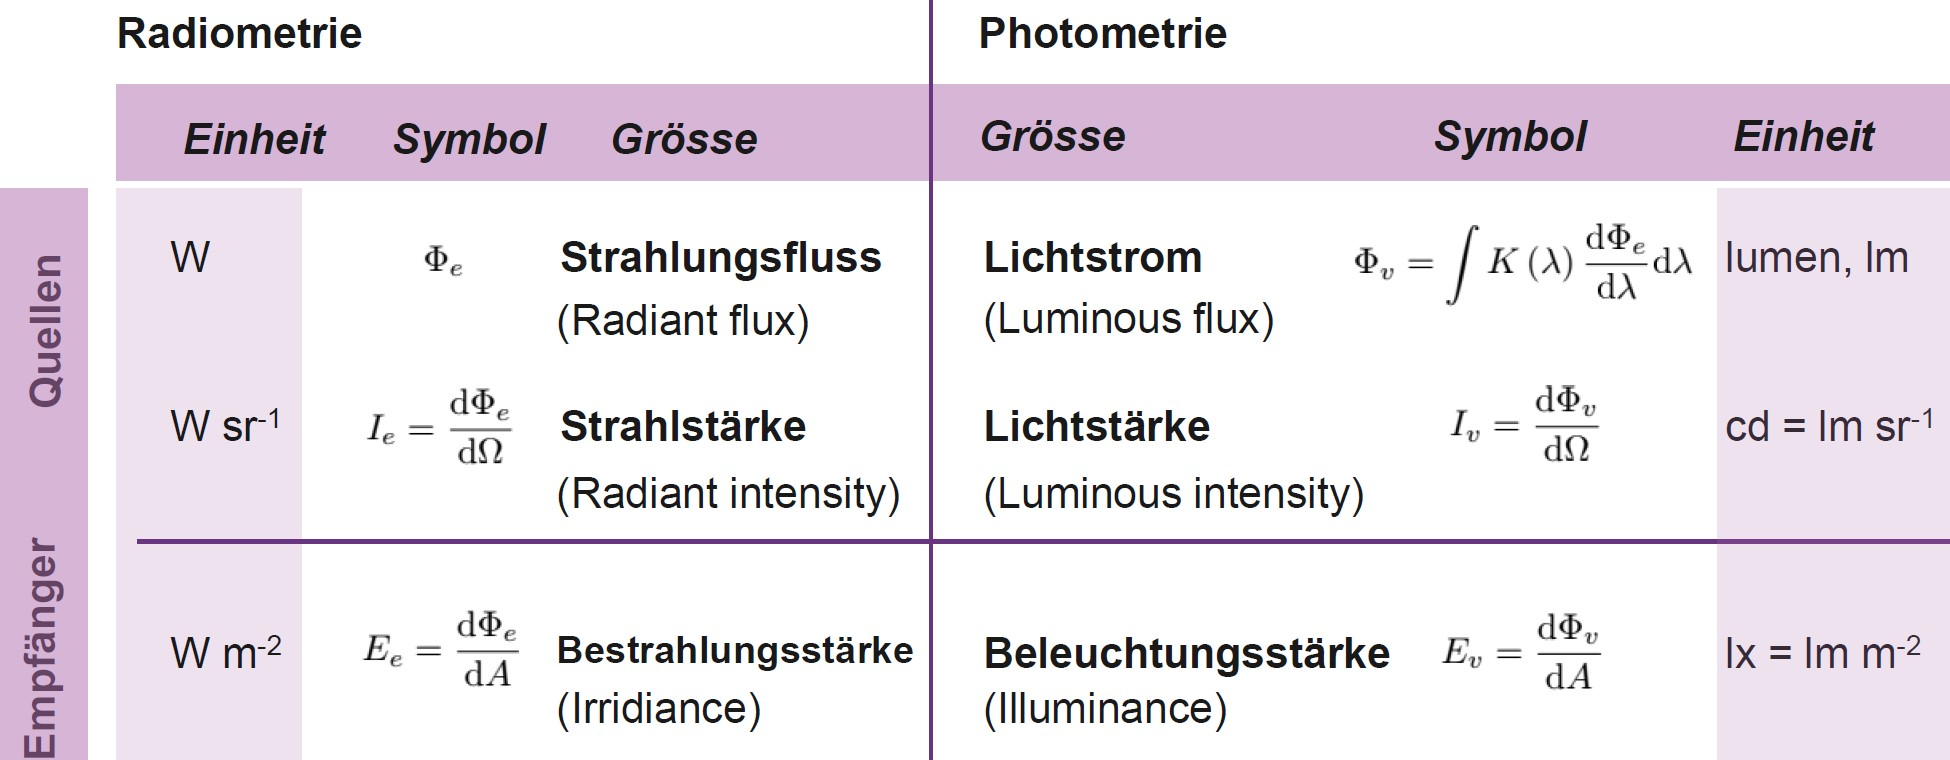
\includegraphics[width=\linewidth]{Bilder/Wellen-Optik/radiometrie_photometrie}




\subsection{Raumwinkel}

\subsubsection{Winkel in der Ebene (Radiant)}

\begin{minipage}{0.4\linewidth}
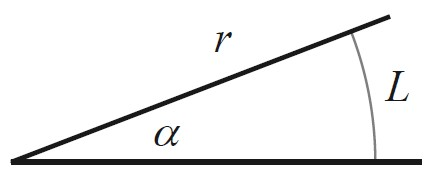
\includegraphics[width=\linewidth]{Bilder/Wellen-Optik/winkel_ebene}
\end{minipage}
\hfill
\begin{minipage}{0.48\linewidth}
Länge des Bogens auf einem Kreis mit $r = 1 \, \m$ 

$$ \boxed{ \alpha = \frac{L}{r}  } $$ 

Vollkreis: $2 \, \pi$ \qquad $[\alpha] = \mathrm{rad}$ 
\end{minipage}


\subsubsection{Winkel im Raum (Steradiant)}

\begin{minipage}{0.35\linewidth}
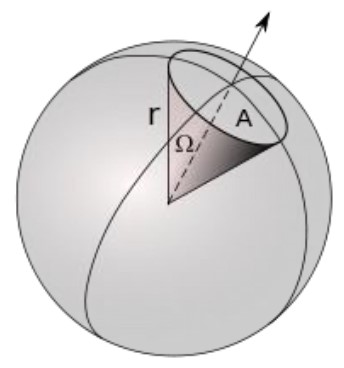
\includegraphics[width=\linewidth]{Bilder/Wellen-Optik/winkel_raum}
\end{minipage}
\hfill
\begin{minipage}{0.62\linewidth}
Aufgespannte Fläche, projiziert auf eine Kugel mit $r = 1 \, \m$

$$ \boxed{ \Omega = \frac{A}{r^2} = \frac{A}{1 \m^2} } $$

Kugel: $4 \, \pi$ \qquad $[\Omega] = \mathrm{sr}$ 
\end{minipage}

% \vfill\null
% \columnbreak




%\subsection{Lichtgeschwindigkeit}

%\subsubsection{Messung nach Romer}

%\subsubsection{Messung nach Fizeau}



\subsection{Reflexionsgesetz}

\begin{minipage}{0.44\linewidth}
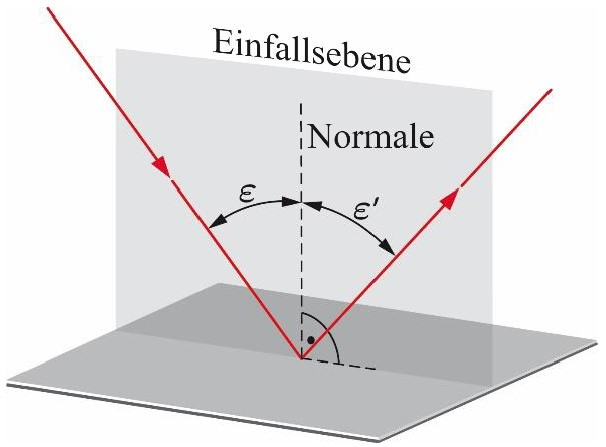
\includegraphics[width=\linewidth]{Bilder/Wellen-Optik/reflexionsgesetz}
\end{minipage}
\hfill
\begin{minipage}{0.48\linewidth}
Einfallswinkel = Ausfallswinkel \\

$$ \boxed{ \varepsilon = \varepsilon' } $$
\end{minipage}



\subsubsection{Grenzflächen von Reflexionen}

\begin{minipage}{0.4\linewidth}
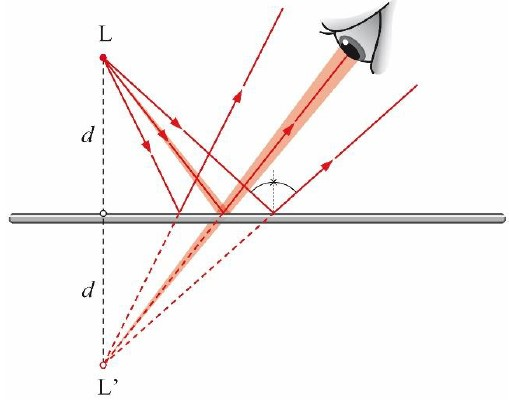
\includegraphics[width=\linewidth]{Bilder/Wellen-Optik/reflexion} \\
\\
\end{minipage}
\hfill
\begin{minipage}{0.58\linewidth}
	\begin{tabular}{ll}
		$L$ & \textbf{reelles Bild} \\
			& Bild, welches auf Schirm \\
			& abgebildet werden kann \\ 
			\\
		$L'$& \textbf{virtuelles Bild} \scriptsize(Spiegelbild von $L$)\normalsize\\
			& Bild, welches nicht auf Schirm \\
			& abgebildet werden kann \\
	\end{tabular}
\end{minipage}

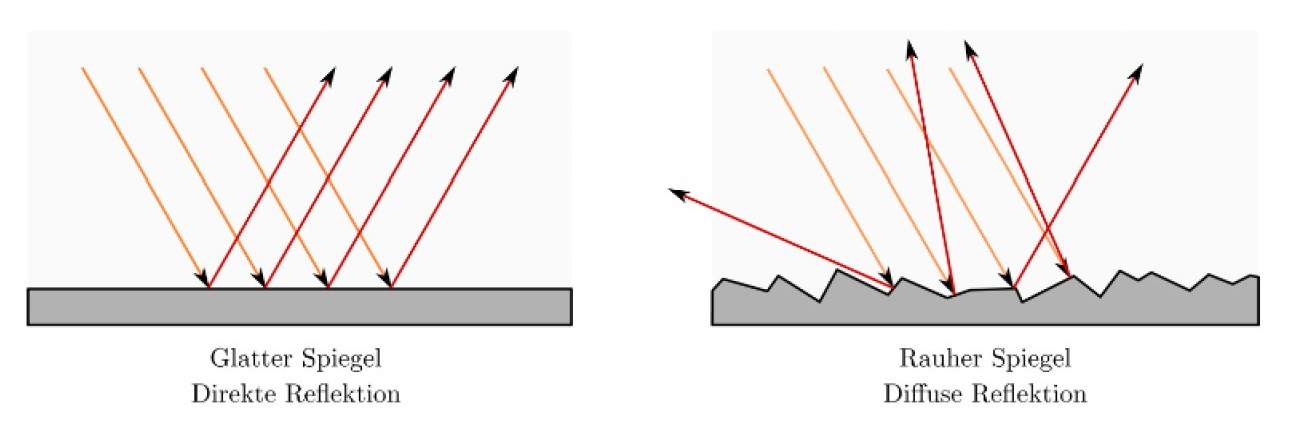
\includegraphics[width=\linewidth]{Bilder/Wellen-Optik/rau-glatt.jpg}

\subsection{Reflexionen - Spezialfälle}

\begin{tabular}{ll}
Brennpunkt $F$ & Brennpunkt (Fokus) ist der Punkt, in dem parallel \\
 		       & zur optischen Achse auf einen Spiegel oder eine \\
 		       & Linse einfallende Stahlen sich schneiden \\
 		   \\
Brennweite $f$ & Abstand des Brennpunktes von der Linse bzw. \\
		       & dem Spiegel
\end{tabular}


\subsubsection{Parabolspiegel}
Parallel einfallende Strahlen werden in einem Punkt fokussiert \\


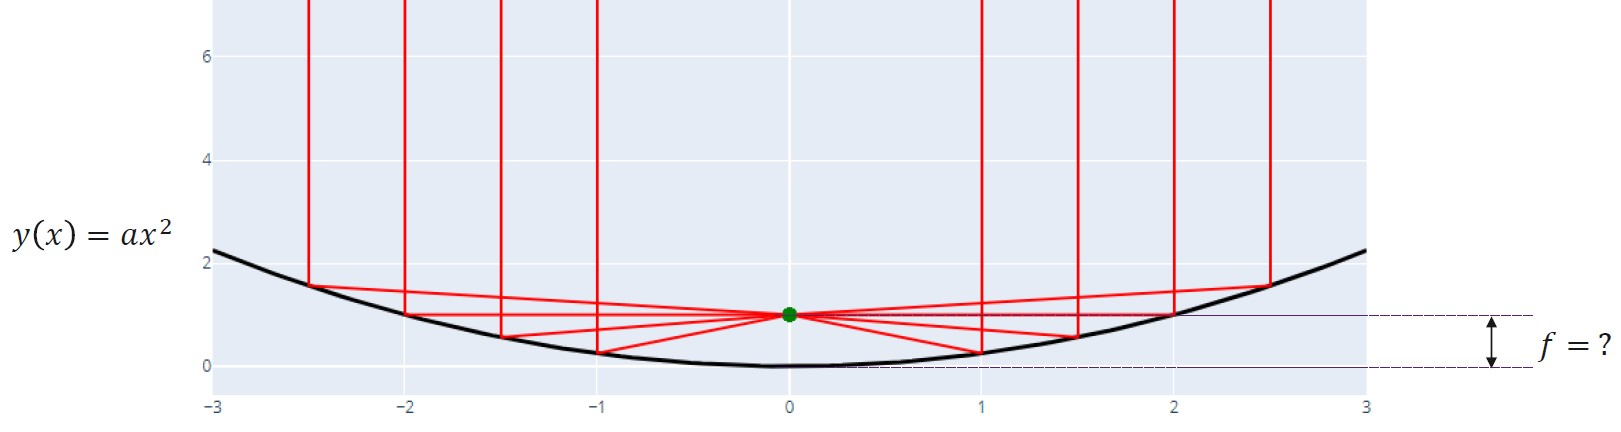
\includegraphics[width=0.9\linewidth]{Bilder/Wellen-Optik/parabolspiegel} \\

\begin{minipage}{0.48\linewidth}
$$ \boxed{ y(x) = a \, x^2 } $$ 
\end{minipage}
\hfill
\begin{minipage}{0.48\linewidth}
$$ \boxed{ f = \frac{1}{4 \, a} } $$
\end{minipage}


% \vfill\null
% \columnbreak



\subsubsection{Elliptischer Spiegel}

Konzentration von Energie in einem nicht zugänglichen Punkt \\

\begin{minipage}{0.48\linewidth}
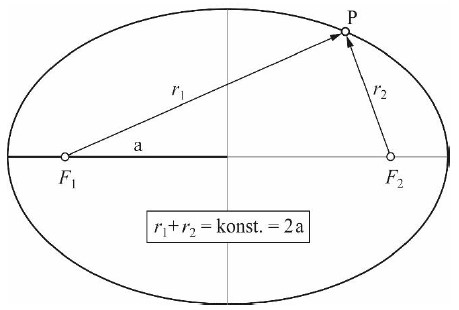
\includegraphics[width=\linewidth]{Bilder/Wellen-Optik/elliptischer_spiegel} 
\end{minipage}
\hfill
\begin{minipage}{0.48\linewidth}
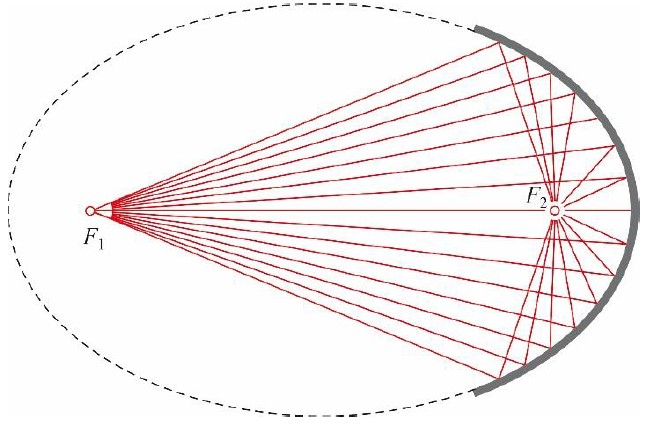
\includegraphics[width=\linewidth]{Bilder/Wellen-Optik/elliptischer_spiegel_2} 
\end{minipage}

$$ \boxed{ y(x) = \frac{x^2}{a^2} + \frac{y^2}{b^2} } $$




\subsubsection{Hyperbolischer Spiegel}

Objekt in Spiegel versetzen \\

\begin{minipage}{0.4\linewidth}
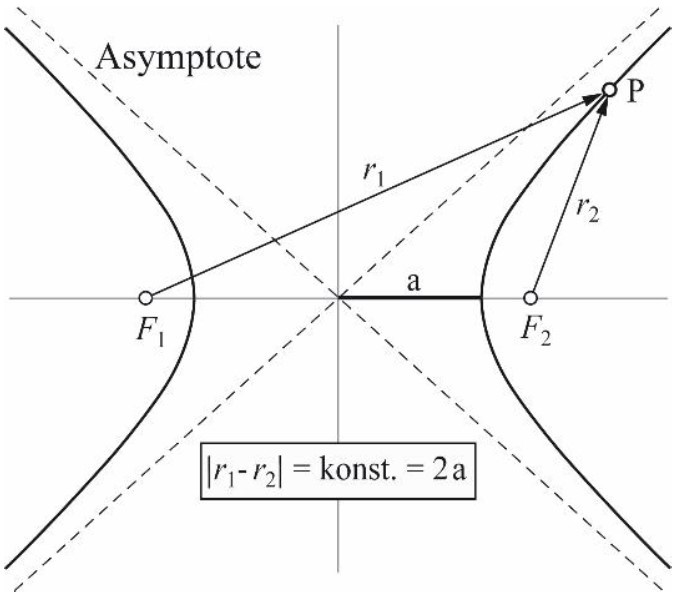
\includegraphics[width=\linewidth]{Bilder/Wellen-Optik/hyperbolischer_spiegel} 
\end{minipage}
\hfill
\begin{minipage}{0.48\linewidth}
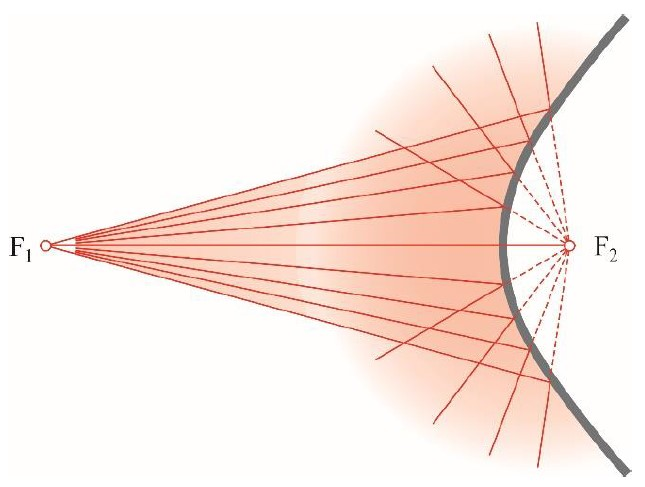
\includegraphics[width=\linewidth]{Bilder/Wellen-Optik/hyperbolischer_spiegel_2} 
\end{minipage}

$$ \boxed{ \frac{x^2}{a^2} - \frac{y^2}{b^2} = 1} $$



\subsubsection{Sphärische Spiegel}

Paralell einfallende Stahlen werden nicht mehr in einem Punkt  \\
fokussiert (Katakaustik) \\
\\
Da die achsnahen Strahlen nach der Reflexion annähernd durch einen Punkt gehen, wird
dieser Punkt wieder Brennpunkt $F$ genannt. \\



\begin{minipage}{0.4\linewidth}
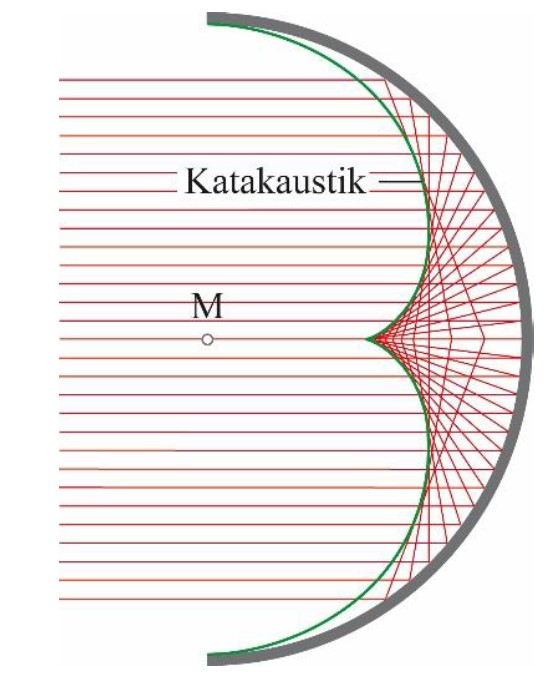
\includegraphics[width=0.8\linewidth]{Bilder/Wellen-Optik/sphaerischer_spiegel_2} 
\end{minipage}
\hfill
\begin{minipage}{0.4\linewidth}
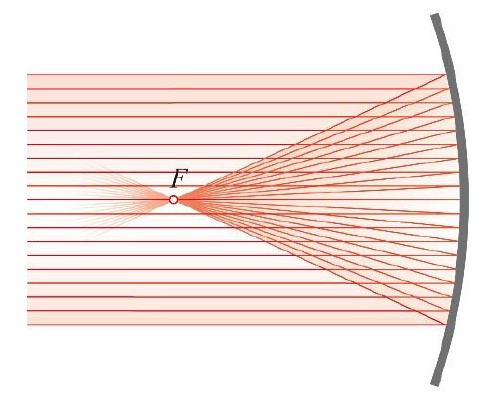
\includegraphics[width=\linewidth]{Bilder/Wellen-Optik/sphaerischer_spiegel} 
\end{minipage}

$$ \boxed{ f = \frac{r}{2} } $$

\begin{tabular}{lll}
$f$ & Brennweite &  $[f] = \m$ \\
$r$ & Krümmungsradius des Spiegels & $[r] = \m$ \\
\end{tabular}


% \vfill\null
% \columnbreak



\subsection{Brechung}

Fällt ein Lichtstrahl auf die Grenzfläche zweier Medien, so dringt ein Teil des einfallenden Lichtes in das zweite Medium ein. \\
Die auftrentende Richtungsänderung wird als \textbf{Brechung} bezeichnet. \\
Der in das zweite Medium eindringende Strahl wird \textbf{gebrochener Strahl} genannt.




\subsubsection{Brechungsgesetz / Geschwindigkeit}

\begin{minipage}{0.48\linewidth}
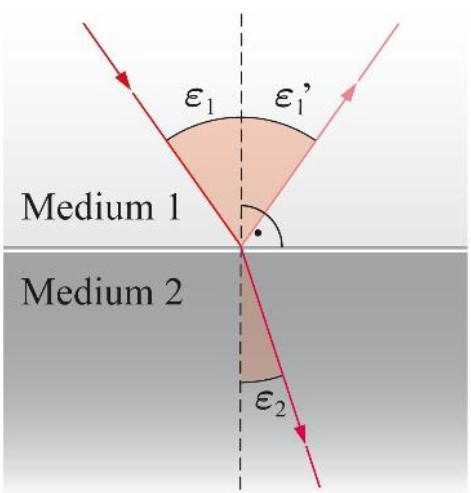
\includegraphics[width=0.7\linewidth]{Bilder/Wellen-Optik/brechung} \\
$n_2 > n_1$  \\
\end{minipage}
\hfill
\begin{minipage}{0.48\linewidth}
$$ \boxed{ \frac{\sin(\varepsilon_1)}{\sin(\varepsilon_2)} = \frac{n_2}{n_1}  } $$

$$ \boxed{ v_i = \frac{c}{n_i}  } $$

Je grösser $n$, desto grösser die \\
Ablenkung und desto kleiner $\varepsilon$ \\

\end{minipage}


\begin{tabular}{c l c}
	$\varepsilon_i$ & Winkel zur Normalen & $[\varepsilon_i] =$° \\
	$n_i$ & Brechungsindex & $[n_i] = 1$ \\
	$v_i$ & Geschwindigkeit im Medium $n_i$ & $[v_i] = \mathrm{\frac{m}{s}}$ \\
	$c$ & Lichtgeschwindigkeit $c = 300 \cdot 10^6 \, \mathrm{\frac{m}{s}}$ & $[c] = \mathrm{\frac{m}{s}}$ \\
\end{tabular}

\subsubsection{Anwendung: Glasfaser}

Der Lichtstrahl bliebt in der Kernzone (Medium 1) gefangen, da diese einen grösseren Brechungsindex hat als die Mantelschicht (Medium 2) \\

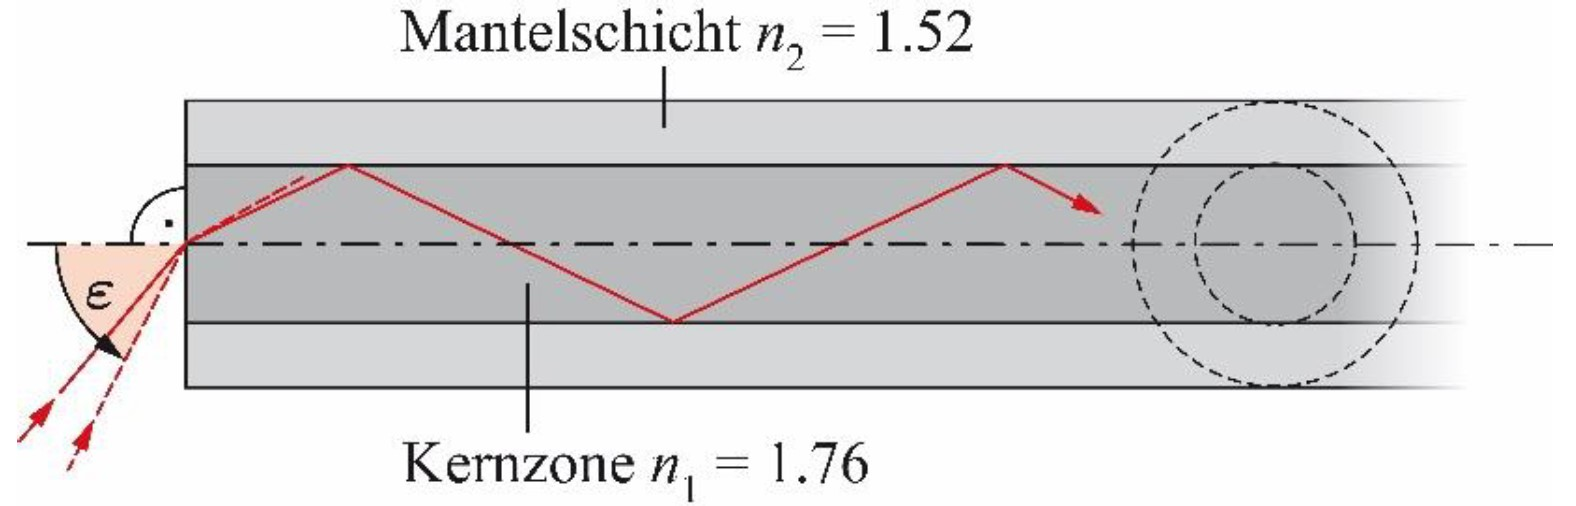
\includegraphics[width=0.75\linewidth]{Bilder/Wellen-Optik/glasfaser}

\textbf{Extremfall} (\textit{Numerical Aperture} NA = $nsin\theta_{max}$):\\
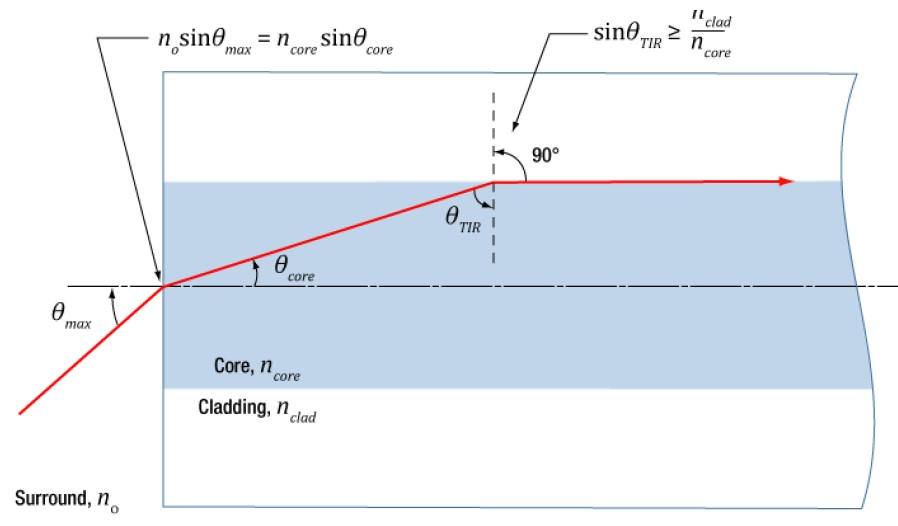
\includegraphics[width=0.8\linewidth]{Bilder/Wellen-Optik/glasfaser-2.jpg}

\begin{center}
	$ \boxed{n_0sin\theta_{max} = \sqrt{n^2_{core} - n^2_clad}} $ 
\end{center}






\subsubsection{Totalreflexion}

Der Einfallswinkel $\varepsilon_1$ kann nicht grösser als 90° sein. \\
Für $\varepsilon_1 = 90$° berechnet sich $\varepsilon_2 = \varepsilon_g$ aus: 

%$$ \frac{sin(\varepsilon_1)}{sin(\varepsilon_1)} = \frac{1}{sin(\varepsilon_g)} = \frac{n_2}{n1} $$

$$ \boxed{\varepsilon_g = \arcsin \left( \frac{n_1}{n_2} \right)} $$


Für den Grenzfall von $\varepsilon_1 > 90$° wird der gesamte Stahl reflektiert. \\



\begin{minipage}{0.35\linewidth}
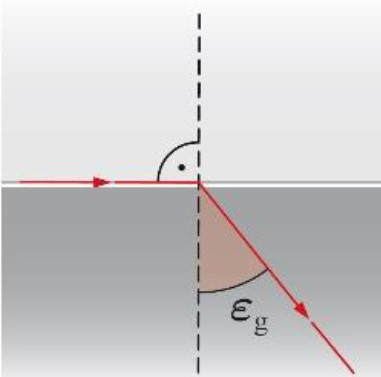
\includegraphics[width=\linewidth]{Bilder/Wellen-Optik/totalreflexion} 
\end{minipage}
\hfill
\begin{minipage}{0.35\linewidth}
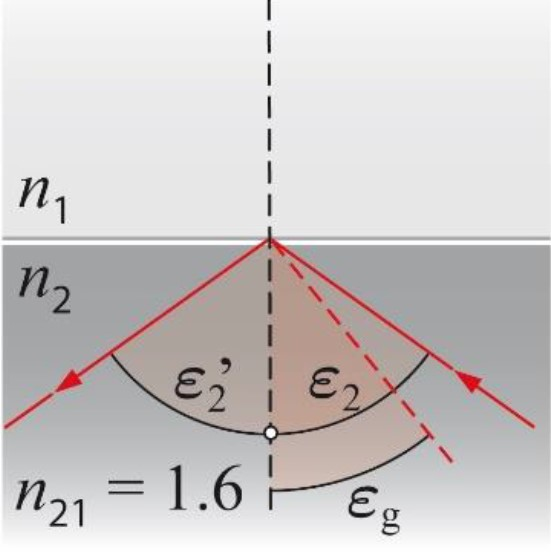
\includegraphics[width=\linewidth]{Bilder/Wellen-Optik/totalreflexion_2} 
\end{minipage}

% \vfill\null
% \columnbreak


\subsubsection{Brechung an ebenen Grenzflächen}

Ein Lichtstrahl wird verschoben bzw. in eine beliebige Richtung geändert\\


\begin{minipage}{0.4\linewidth}
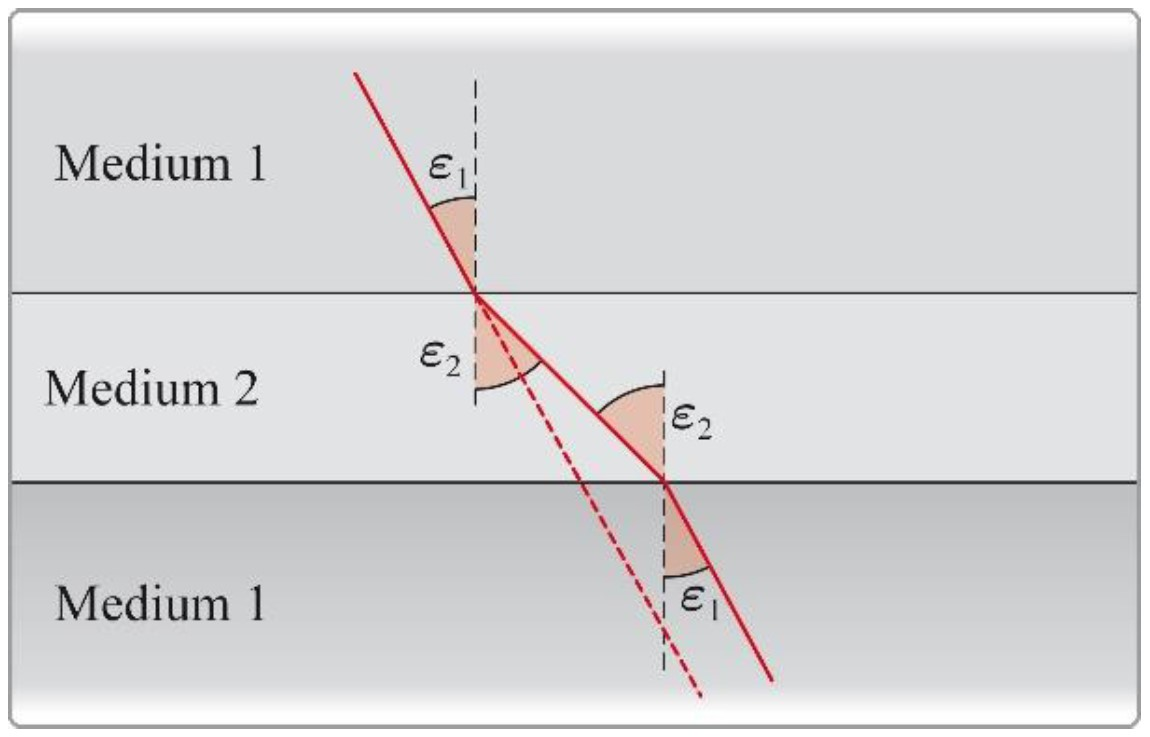
\includegraphics[width=\linewidth]{Bilder/Wellen-Optik/verschiebung_lichtstrahl} 
\end{minipage}
\hfill
\begin{minipage}{0.4\linewidth}
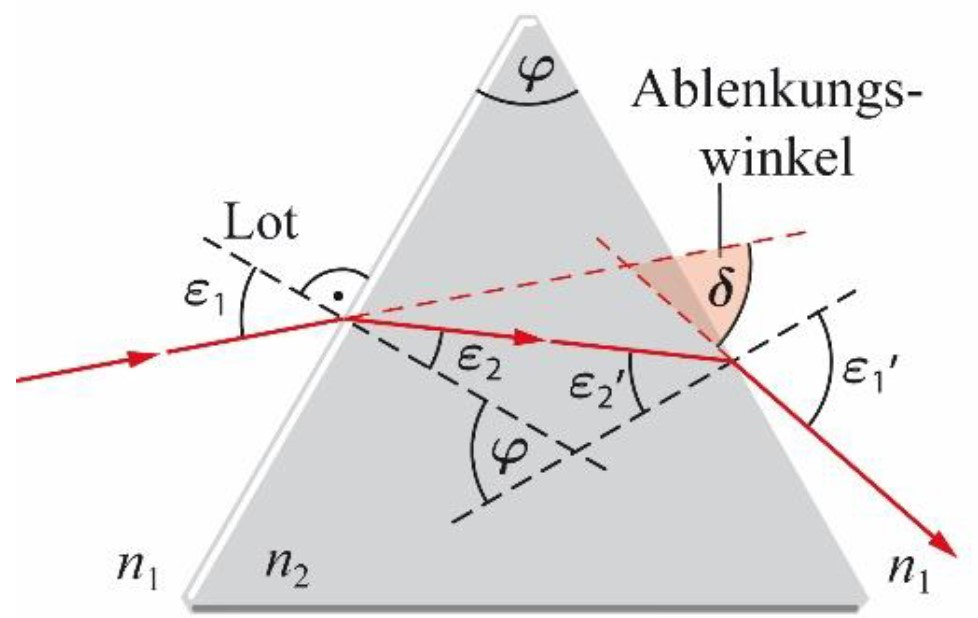
\includegraphics[width=\linewidth]{Bilder/Wellen-Optik/prisma} 
$$\boxed{n = \frac{\sin{\epsilon_1}}{\sin{\epsilon_2}} = \frac{\sin{\frac{\varphi + \delta}{2}}}{\sin{\frac{\varphi}{2}}}}$$
\end{minipage}



\subsubsection{Brechung an gekrümmten Flächen}

DIE Anwendung der Brechung ist eine Linse.


\subsubsection{Linsentypen}

\begin{minipage}{0.3\linewidth}
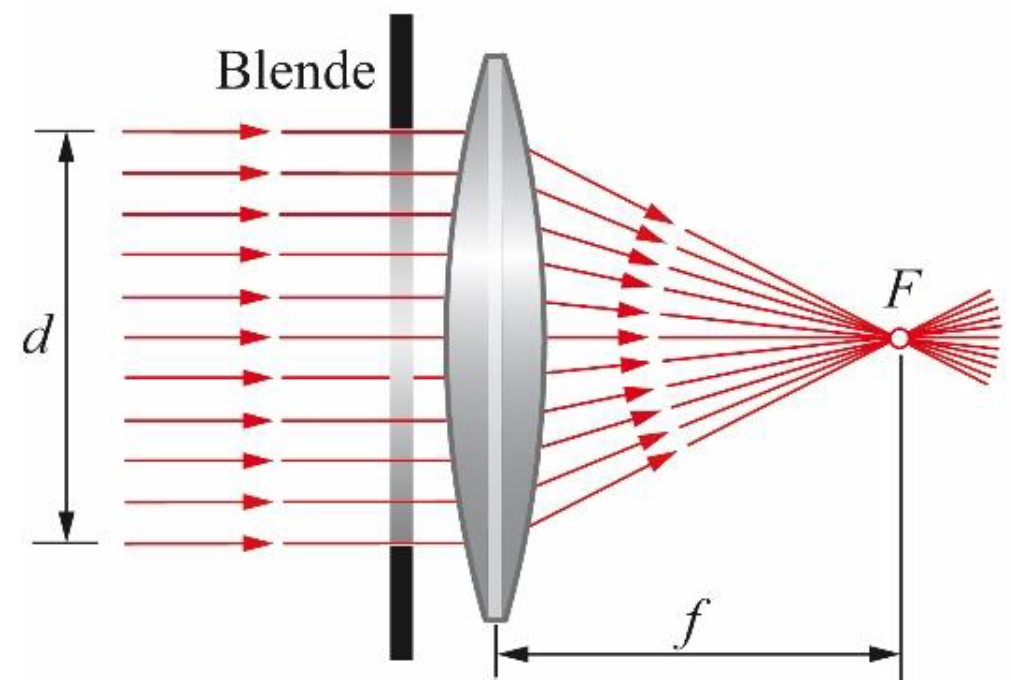
\includegraphics[height=2.0cm]{Bilder/Wellen-Optik/sammellinse} \\
\center{Sammellinse} \\
\end{minipage}
\hfill
\begin{minipage}{0.3\linewidth}
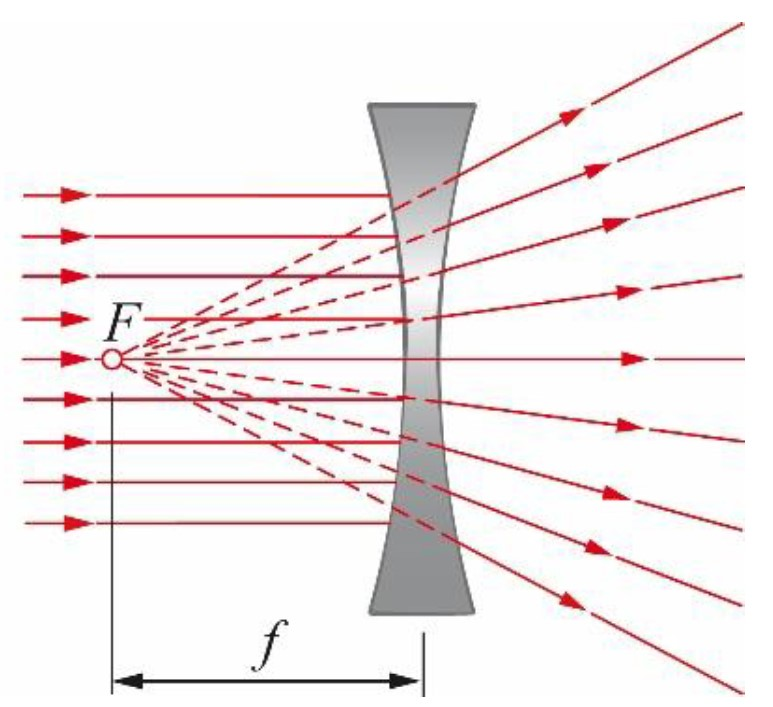
\includegraphics[height=2.0cm]{Bilder/Wellen-Optik/zerstreuungslinse}
\center{Zerstreuungslinse} \\
\end{minipage}
\hfill
\begin{minipage}{0.3\linewidth}
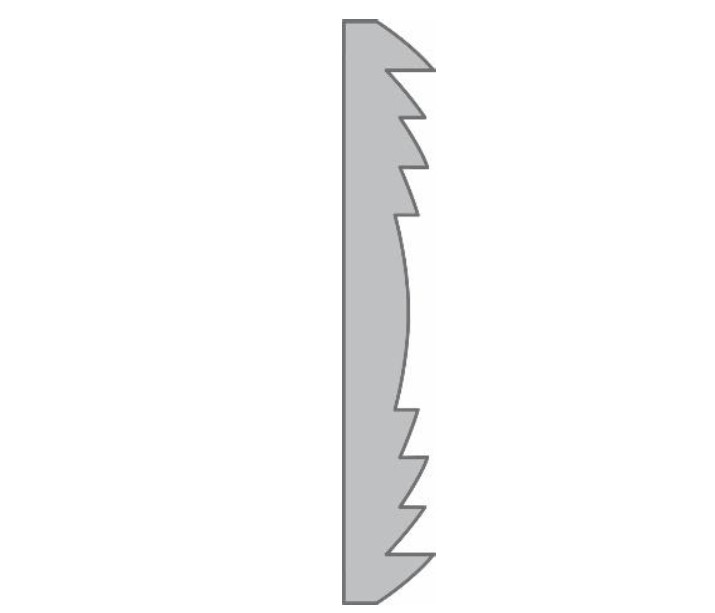
\includegraphics[height=2.0cm]{Bilder/Wellen-Optik/fresnellinse}
\center{Fresnellinse} \\
\end{minipage}

\vspace{0.2cm}

\textbf{Fresnellinse:} Es kann vermieden werden, dass die Linse eine übermässige Dicke aufweist. 



\subsubsection{Beispiel mit zwei Linsen}

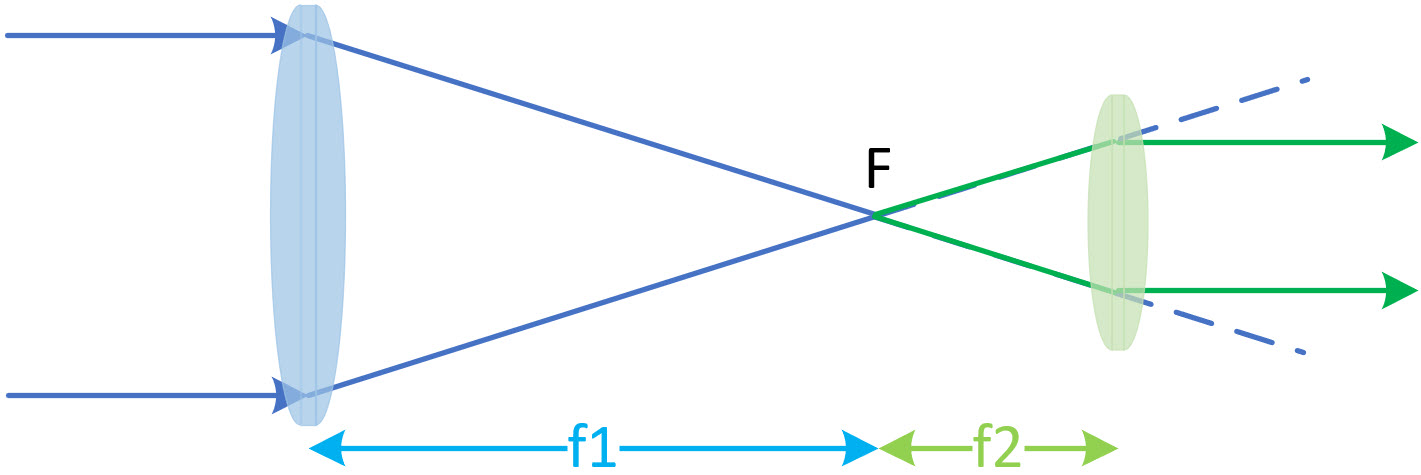
\includegraphics[width=0.9\linewidth]{Bilder/Wellen-Optik/linsen}\\

Rechts gibt es ein kleineres Bild als links.

\subsubsection{Typische Brechungswerte}

\begin{tabular}{| l | c |}
	\hline
	\textbf{Material} & \textbf{Brechungsindex $n$ für $\lambda$ = 589 nm} \\ \hline
	Luft (Normalbed.)        & 1.000'292 \\ \hline
	Helium (Normalbed.)      & 1.000'034'911 \\ \hline
	Wasser (20°C)            & 1.33 \\ \hline
	Glycerin                 & 1.47 \\ \hline
	Quarzglas                & 1.54 \\ \hline
	Plexiglas                & 1.51 \\ \hline
	Kronglas                 & 1.52 \\ \hline
	Brillenglas (Kunststoff) & bis 1.76 \\ \hline
	Diamant                  & 2.42 \\ \hline
\end{tabular}



\subsection{Dispersion}
\label{Dispersion Optik}


Der \textbf{Brechungsindex} eines Mediums ist eine \textbf{Funktion \\
der Wellenlänge:} $n = n(\lambda)$ \\
Diese Wellenlängenabhängigkeit wird als \textbf{Dispersion} bezeichnet \\


\begin{minipage}{0.48\linewidth}
$$ \boxed{ n^2(\lambda) = 1 + \frac{A}{ \frac{1}{\lambda_0^2} -  \frac{1}{\lambda^2} }  }  $$
\end{minipage}
\hfill
\begin{minipage}{0.48\linewidth}
$$ \boxed{ n^2(f) = 1 + \frac{A'}{f_0^2 - f^2}  }  $$
\end{minipage}


\subsubsection{Abbe Zahl $V$}

Gibt an, wie stark dispersiv ein Material ist \\
Grosse Abbe-Zahl $\rightarrow$ wenig dispersives Material




\subsection{Abbildungen}

\subsubsection{Konstruktions-Anweisung}

Man benutzt zwei der drei Hauptstrahlen: \\

\begin{tabular}{l l c l}
1. & Paralleler Strahl & $\rightarrow$ & Brennpunkt \\
2. & Mittelpunkt-Strahl & $\rightarrow$ & mit gleichem Winkel zurück \\
3. & Brennpunkt-Strahl & $\rightarrow$ & Paralleler Strahl \\
\\
\end{tabular}



\begin{minipage}{0.48\linewidth}
\center{ \textbf{reelles Bild} }
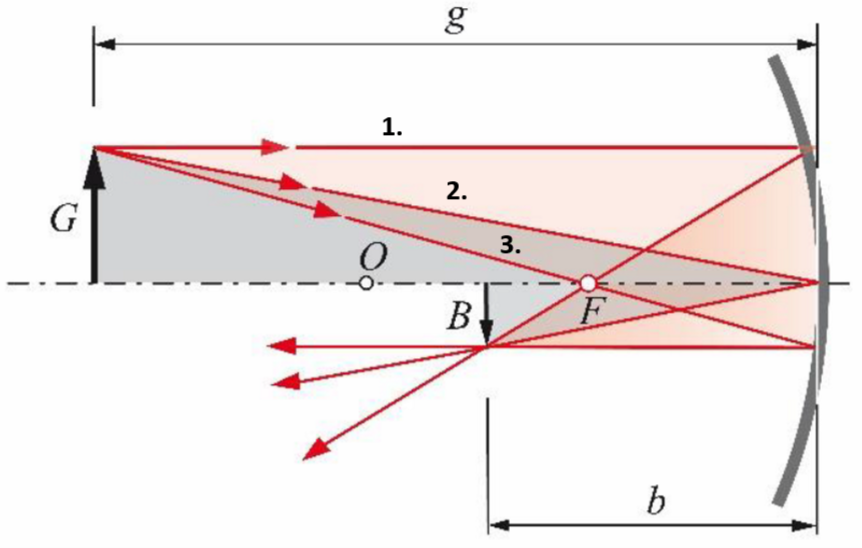
\includegraphics[width= 0.9\linewidth]{Bilder/Wellen-Optik/reelles_bild} \\
\end{minipage}
\hfill
\begin{minipage}{0.48\linewidth}
\center{ \textbf{virtuelles Bild} }
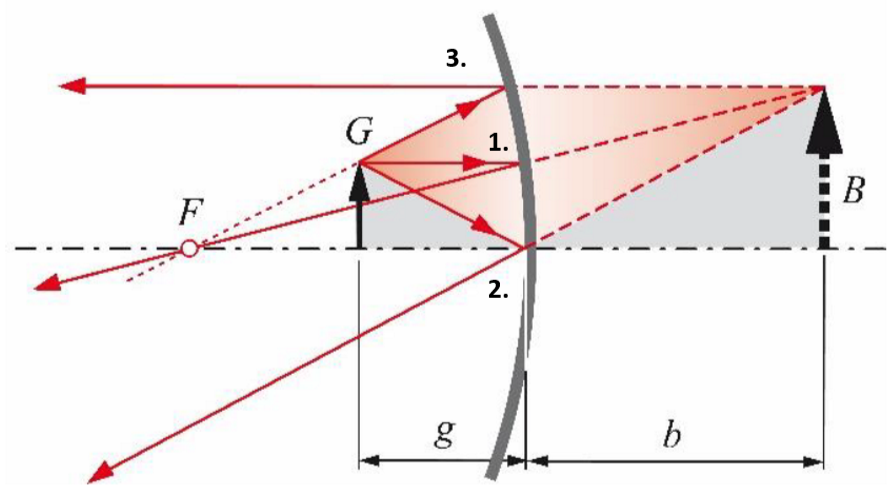
\includegraphics[width= 0.9\linewidth]{Bilder/Wellen-Optik/virtuelles_bild} \\
\end{minipage}


$B$ wird als \textbf{reeller Bildpunkt} bezeichnet, wenn sich die austretenden Strahlen schneiden. \\
\\
$B$ wird als \textbf{virtueller Bildpunkt} bezeichnet, wenn sich nur die Verlängerungen der austretenden Strahlen schneiden. 


\subsubsection{Terminologie}

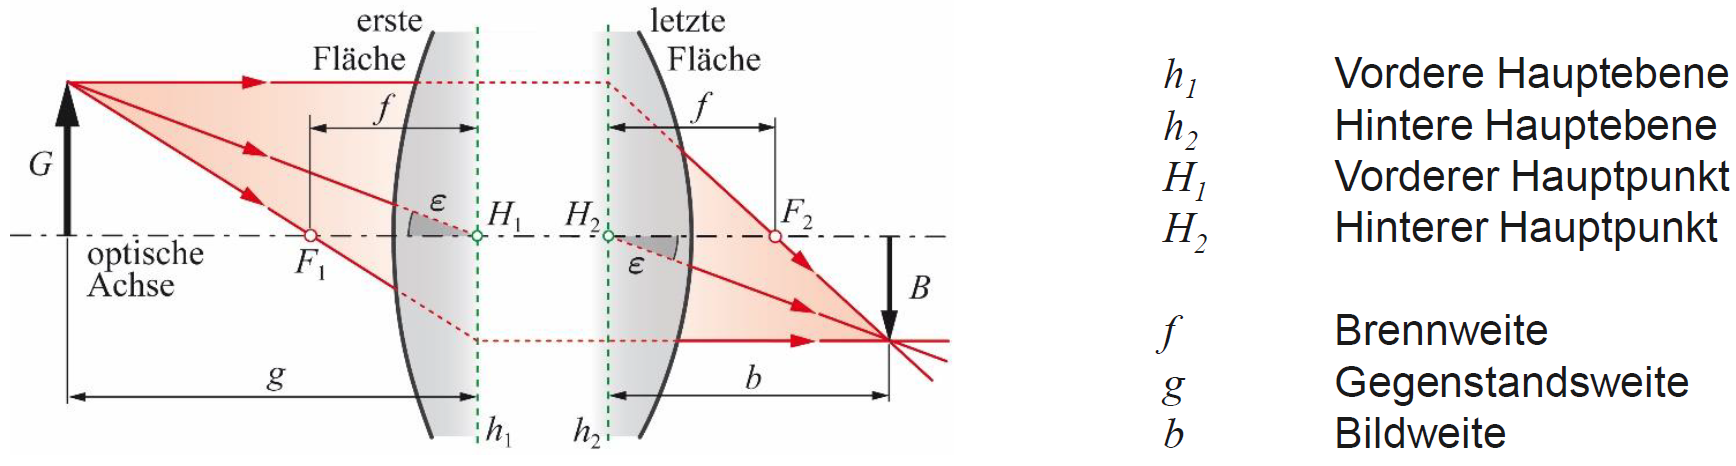
\includegraphics[width=0.9\linewidth]{Bilder/Wellen-Optik/terminologie} \\

Die \textbf{Öffnungsblende} oder \textbf{Aperturblende} begrenzt das in das System einfallende Lichtbündel \small (Irisblenden, Linsenfassungen)\normalsize \\
\\
Die \textbf{Feldblende} begrenzt das Bildfeld. Sie legt den Ausschnitt der Objektebene fest, der abgebildet wird. \small (Foto-, Filmkamera: Formatrahmen) \normalsize


\subsubsection{Beispiel: Abbildungen bei zwei Sammellinsen}

\begin{minipage}{0.48\linewidth}
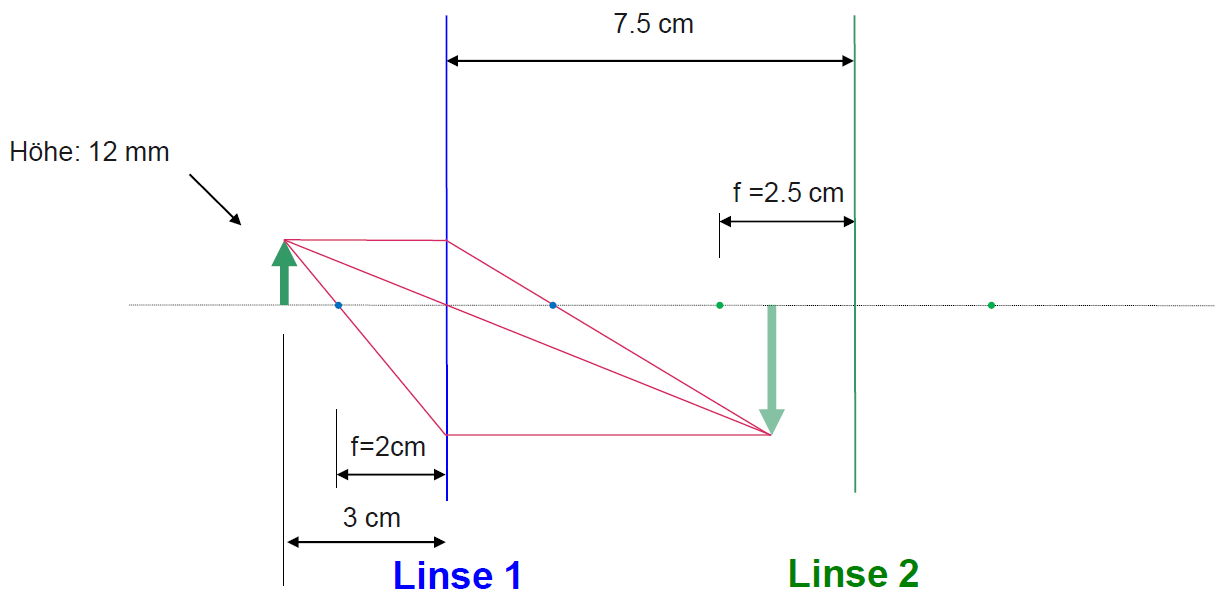
\includegraphics[width=0.98\linewidth]{Bilder/Wellen-Optik/zwei_sammellinsen_1} 
\end{minipage}
\hfill
\begin{minipage}{0.48\linewidth}
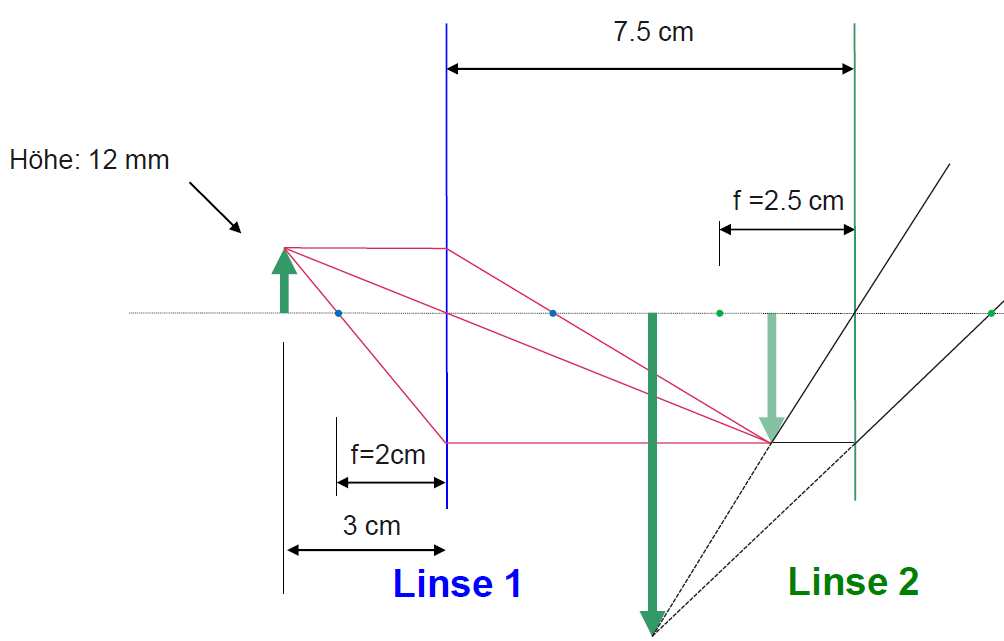
\includegraphics[width=0.98\linewidth]{Bilder/Wellen-Optik/zwei_sammellinsen_2} 
\end{minipage}



% \vfill\null
% \columnbreak


\subsection{Abbildungsgleichungen}
\textbf{Ein Bild ist scharf dargestellt, wenn die Abbildungsgleichung erfüllt ist!} \\



\begin{minipage}{0.48\linewidth}
	\begin{center}
		\textbf{Abbildungsgleichung} \\
		$$ \boxed{ \frac{1}{b} + \frac{1}{g} = \frac{1}{f} } $$
	\end{center}
\end{minipage}
\hfill
\begin{minipage}{0.48\linewidth}
	\begin{center}
		\textbf{Newtonsche Abb.-Gleichung} \\
		$$ \boxed{ x_b \cdot x_g = f^2 } $$
	\end{center}
\end{minipage}


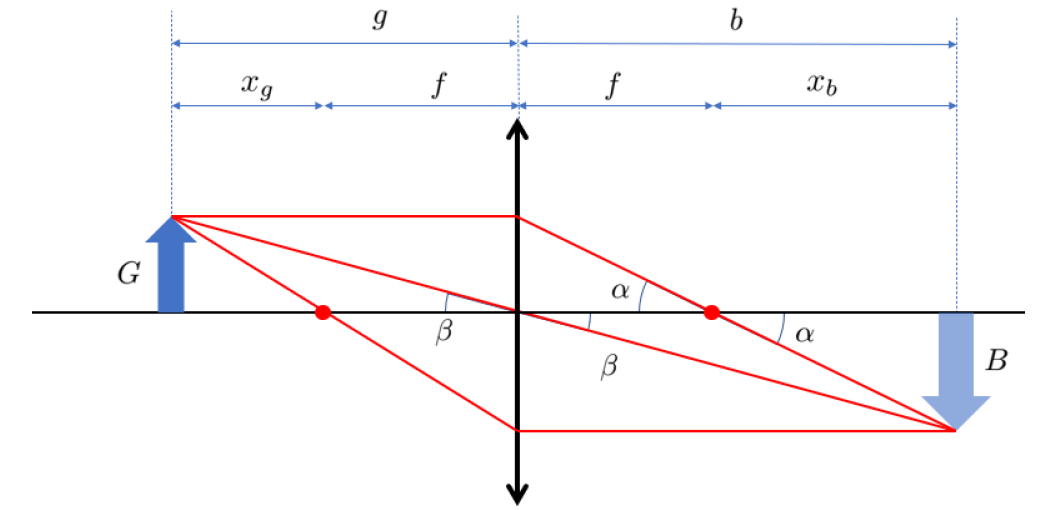
\includegraphics[width=\linewidth]{Bilder/Wellen-Optik/abbildungsgleichung}
\begin{minipage}{0.50\linewidth}
	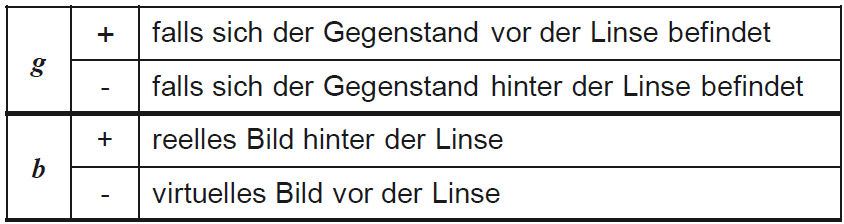
\includegraphics[width=\linewidth]{Bilder/Wellen-Optik/abbildungsgleichung-1.png}
\end{minipage}
\hfill
\begin{minipage}{0.48\linewidth}
	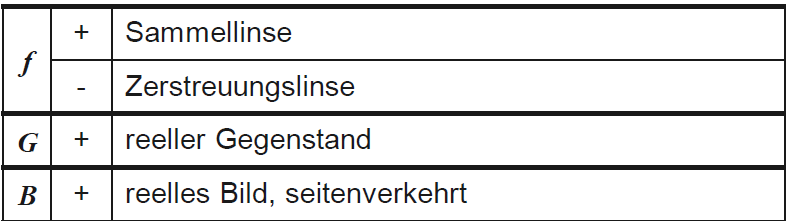
\includegraphics[width=\linewidth]{Bilder/Wellen-Optik/abbildungsgleichung-2.png}
\end{minipage}

\textcolor{blue}{ \textbf{Hinweis:} Ein Spiegel hat eine Brennweite von $f = \infty$ \\
$\Rightarrow$ Vereinfachung der Abbildungsgleichung!}


\subsubsection{Vergrösserungsverhältnis}

\begin{minipage}{0.48\linewidth}
$$ \boxed{ V = \frac{B}{G} = \frac{b}{g} } $$
\end{minipage}
\hfill
\begin{minipage}{0.48\linewidth}
$$ \boxed{ V_{tot} = V_1 \cdot V_2 } $$ 
\end{minipage}

\vspace{0.2cm}



\begin{tabular}{c l c}
	$V$ & Vergrösserungsverhältnis & $[V] = 1$ \\
	$b$ & Bildweite & $[b] = \m$ \\
	$g$ & Gegenstandsweite & $[g] = \m$ \\
	$B$ & Bildgrösse & $[B] = \m$ \\
	$G$ & Gegenstandsgrösse & $[G] = \m$ \\
	$f$ & Brennweite & $[f] = \m$ 
\end{tabular}




\subsection{Brechkraft $D$}
Die Optiker benutzen nicht die Brennweite sondern die Brechkraft \\
in \textbf{Dioptrie}  \\
Es gilt: $1 \, \mathrm{dpt} = 1 \, \m^{-1}$

$$ \boxed{ D = \frac{1}{f} }$$

% \vfill\null
% \columnbreak



\subsection{Linsenschleifergleichung}

\begin{minipage}{0.52\linewidth}
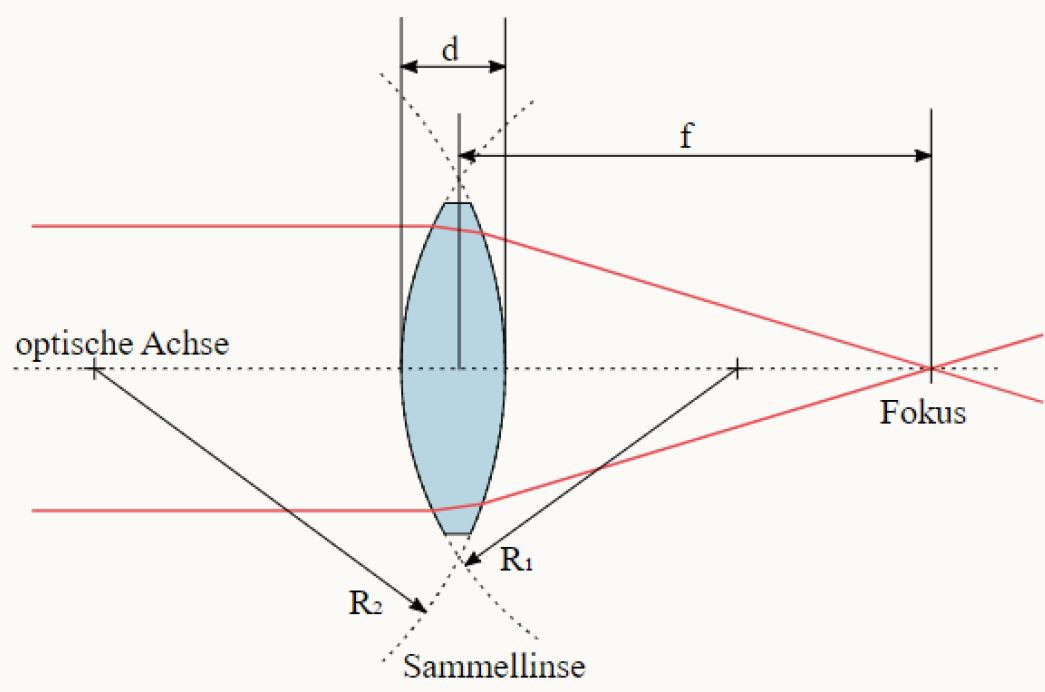
\includegraphics[width=\linewidth]{Bilder/Wellen-Optik/Linsenschleifergleichung}
\end{minipage}
\hfill
\begin{minipage}{0.46\linewidth}
$$\boxed{D = \left(\frac{n_2}{n_1}-1\right) \left(  \frac{1}{R_1} - \frac{1}{R_2} \right)  }$$

\textcolor{blue}{Vorzeichen von $R_i$ beachten!} \\
Beide haben \\
gleiches Vorzeichen, wenn Krümmungsmittelpunkte auf gleicher Seite der Linse liegen
\end{minipage}



\subsubsection{Symmetrische Linsen ($R_1 = R_2$)}

Für symmetrische Linsen gilt:

\begin{minipage}{0.48\linewidth}
$$\boxed{D = (n - 1)\frac{2}{R}}$$ \\
\end{minipage}
\hfill
\begin{minipage}{0.48\linewidth}
$$\boxed{f = \frac{1}{D} = \frac{R}{2}\frac{1}{(n - 1)}} $$ \\
\end{minipage}



\begin{tabular}{c l c}
	$D$ & Brechkraft & $[D] = \mathrm{dpt}$ \\
	$f$ & Brennweite & $[f] = \mathrm{\frac{1}{s} = Hz}$ \\
	$R_i$ & Linsenradius & $[R_i] = \m$ \\
	$n$ & Brechungsindex & $[n] = 1$ \\
\end{tabular}


\subsubsection{Kombination von zwei Linsen}

\begin{minipage}{0.48\linewidth}
	$$ \boxed{\frac{1}{f} = \frac{1}{f_1} + \frac{1}{f_2} - \frac{d}{f_1f_2}} $$
\end{minipage}
\hfill
\begin{minipage}{0.48\linewidth}
	$$ \boxed{f = \frac{f_1f_2}{f_1 + f_2 - d}} $$
\end{minipage}

\subsubsection{Kombination von zwei dünnen Linsen ohne Zwischenraum}

Die Kombination von zwei dünnen Linsen ohne Zwischenraum ist \\
wie folgt definiert:

$$ \boxed{D = D_1 + D_2} $$




\subsection{Konvexe und Konkave Linsen}

\textbf{Konvex:} nach aussen gewölbt

\textbf{Konkav:} nach innen gewölbt

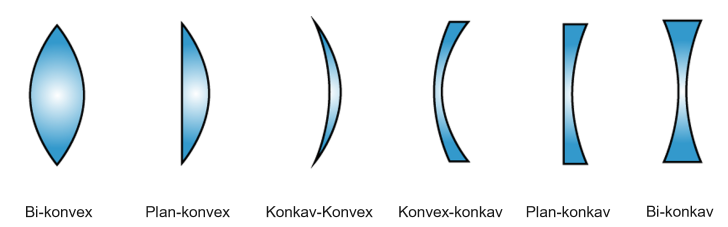
\includegraphics[width=0.9\linewidth]{Bilder/Wellen-Optik/Konvex}

\qquad\qquad Sammellinsen \qquad\qquad\qquad Zerstreuungslinsen



\subsection{Aberration}
Unter dem Begriff Aberration versteht man die Abweichung\\
vom idealisierten Fall. \\

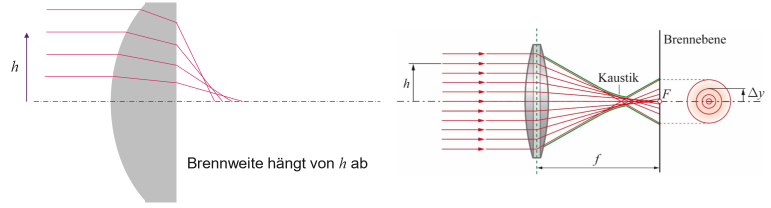
\includegraphics[width=0.9\linewidth]{Bilder/Wellen-Optik/Aberration}



\subsubsection{Astigmatismus}

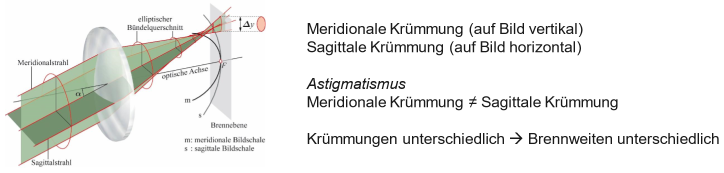
\includegraphics[width=0.9\linewidth]{Bilder/Wellen-Optik/Astigmatismus}





\subsection{Polarisation}


\subsubsection{Lineare Polarisation}

$E_x$ und $E_y$ können \textbf{unterschiedliche Amplituden} haben. \\
Die \textbf{Phasen müssen gleich} sein.\\
\\
EM-Wellen können mit dem Herzsches Gitter oder mit dem \textbf{Brewster Winkel} linear polarisiert werden.

\begin{minipage}{0.48\linewidth}
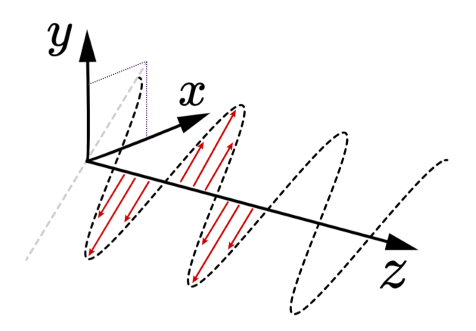
\includegraphics[width=0.9\linewidth]{Bilder/Wellen-Optik/lineare_Polarisation}
\end{minipage}
\hfill
\begin{minipage}{0.48\linewidth}
$$ \boxed{  \vec{E} = \begin{pmatrix} E_x \\  E_y \\  0  \end{pmatrix}  } $$

\center{  $\vec{E}$ kann zu $\vec{0}$ werden }

\end{minipage}




\subsubsection{Brewster Winkel}

Unter dem \textbf{Brewster Winkel} wird nur \textbf{linear polarisiertes Licht} zurückgeworfen. \\
Der ins Medium 2 eindringende Strahl steht dabei \textbf{senkrecht} auf dem reflektierten Strahl \\

\begin{minipage}{0.48\linewidth}
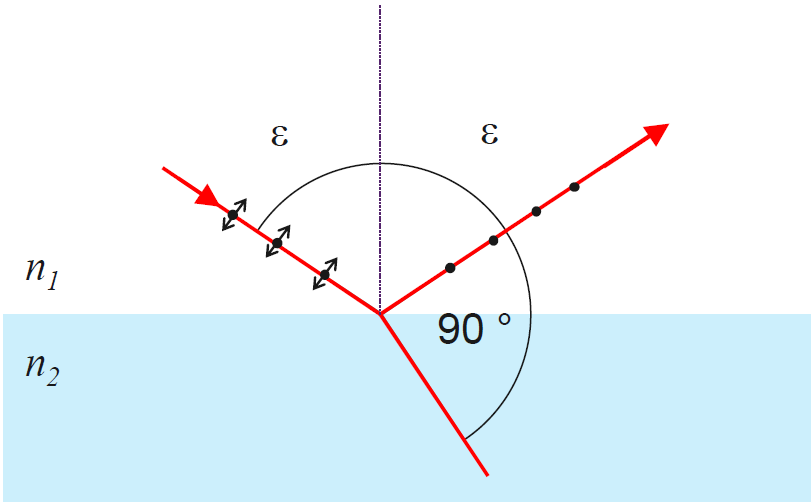
\includegraphics[width=0.75\linewidth]{Bilder/Wellen-Optik/brewster_winkel} \\
$n_1 < n_2$ \\
\end{minipage}
\hfill
\begin{minipage}{0.48\linewidth}
$$ \boxed{  \tan(\varepsilon) = \frac{n_2}{n_1}  }$$

\end{minipage}


% \vfill\null
% \columnbreak



\subsubsection{Zirkulare Polarisation}

$x$ und $y$ Komponenten haben die \textbf{gleiche Amplitude} und eine \textbf{Phasendifferenz von 90°} \\

Positive zirkulare Polarisation $\sigma ^+$ \\
Negative zirkulare Polarisation $\sigma ^-$ \\


\begin{minipage}{0.48\linewidth}
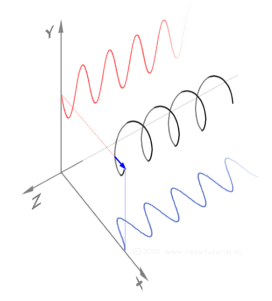
\includegraphics[width=0.8\linewidth]{Bilder/Wellen-Optik/Zirkulare_Polarisation}
\end{minipage}
\hfill
\begin{minipage}{0.48\linewidth}
$$ \boxed{ \vec{E} = \begin{pmatrix} E_0 \cos(2 \pi ft-kz) \\ E_0 \sin(2 \pi ft -kz) \\ 0 \end{pmatrix}  } $$

\center{ $\vec{E}$ kann nicht zu $\vec{0}$ werden }
\end{minipage}

\subsubsection{Elliptische Polarisation}

$x$ und $y$ Komponenten haben \textbf{unterschiedliche Amplituden} und eine \textbf{beliebige Phasendifferenz}.

$$ \boxed{  \vec{E} = \begin{pmatrix} E_0 \cos(2 \pi ft-kz) \\ E_0 \cos(2 \pi ft -kz + \varphi) \\ 0 \end{pmatrix}  } $$





\subsubsection{Doppelbrechung}

Doppelbrechung ist eine anisotropische Eigenschaft von Kristrallen \\
Diese Kristalle haben unterschiedliche Brechungsindizes in unterschiedliche Richtungen \\
\\
Nach einer gewissen Zeit $t$ haben die $x$- und $y$-Komponente einen Phasenunterschied. \\
$\Rightarrow$ $x$ und $y$ bewegen sich unterschiedlich schnell fort \\

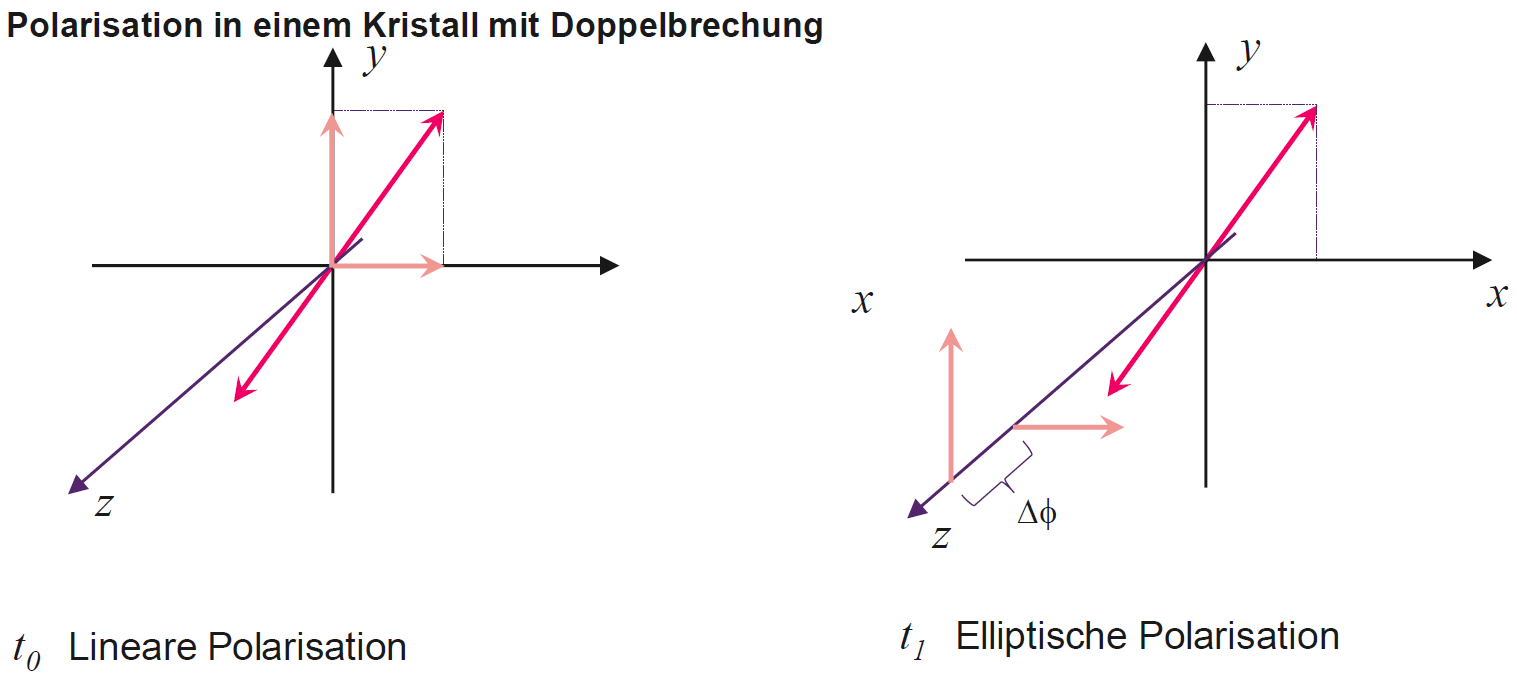
\includegraphics[width=0.8\linewidth]{Bilder/Wellen-Optik/kristall_mit_doppelbrechung}






\subsection{Streuung}

\subsubsection{Diffuse Streuung}

Streuung des Lichts an Teilchen von Dimensionen $d >> \lambda$ \\ 

\begin{minipage}{0.45\linewidth}
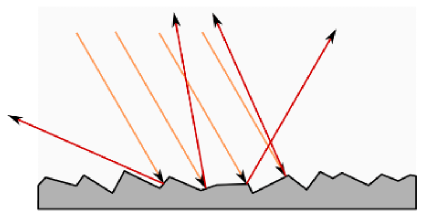
\includegraphics[width=\linewidth]{Bilder/Wellen-Optik/diffuse_streuung}
\end{minipage}
\hfill
\begin{minipage}{0.53\linewidth}

\begin{itemize}
\item Licht als \textbf{Strahlen}
\item Reflexion in alle Richtungen
\item Keine bevorzugte Richtung, \\
	  unabhängig von $\lambda$ 
\item Beispiele:
	\begin{itemize}
		\item Wolken, Nebel 
		\item milchige Lösungen
	\end{itemize}	  
\end{itemize}

\end{minipage}




\subsubsection{Rayleigh-Streuung}

Streuung des Lichts an Teilchen von Dimensionen $d < \lambda$ \\
(atomare Grösse) \\ 

\begin{minipage}{0.38\linewidth}
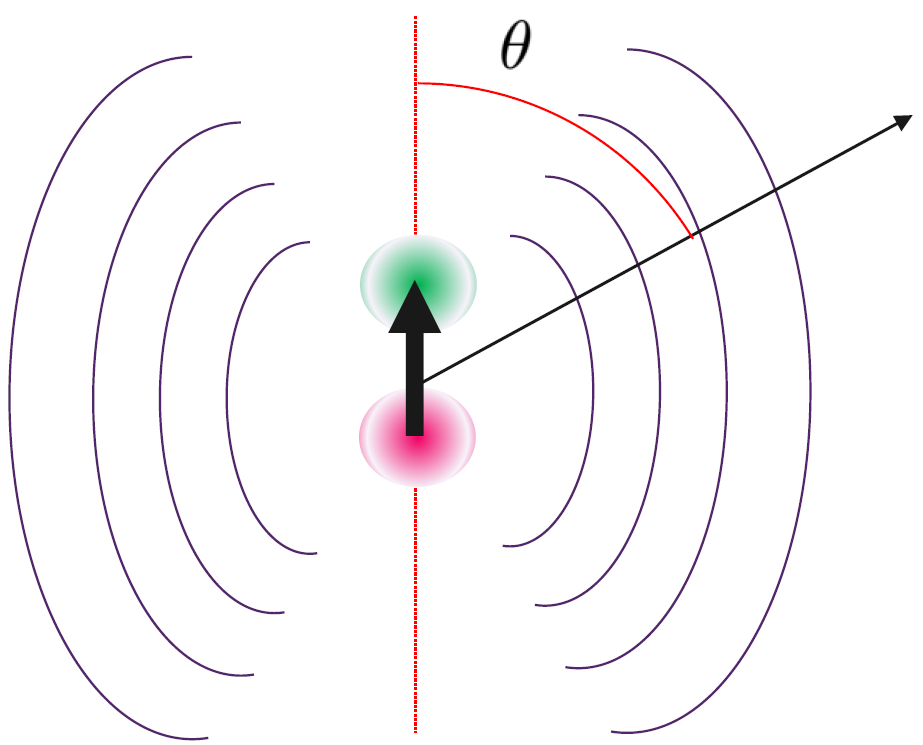
\includegraphics[width=0.9\linewidth]{Bilder/Wellen-Optik/rayleigh_streuung}
\end{minipage}
\hfill
\begin{minipage}{0.58\linewidth}
$$ \boxed{ I(\theta) = A \, f^4 \, \frac{\sin^2 \theta}{r^2} } $$

$\Rightarrow$ hochfrequentes Licht wird viel stärker abgestrahlt! \\

\begin{itemize}

\item Licht als \textbf{Wellen} senkrecht 
	zur Ausbreitungsrichtung 
\item Abstrahlmuster eines Dipols \\
		  %\\
\item Himmel tagsüber blau 
\item Himmel abends rötlich	  

%\endMyItemize
\end{itemize}

\end{minipage}


\subsection{Abbildungssysteme - Auge}

\textbf{Brechzahl Augenlinse}: 1.3\\
\textbf{Tiefe}: $\sim$25mm

\subsubsection{Terminologie des Auges}

\textbf{Sehwinkel $\varepsilon$}

\begin{minipage}{0.48\linewidth}
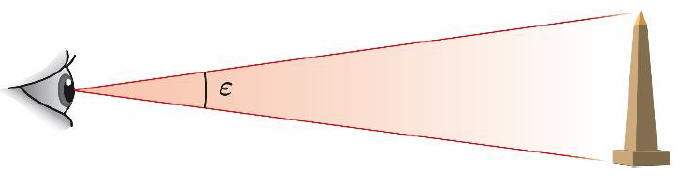
\includegraphics[width=0.9\linewidth]{Bilder/Wellen-Optik/sehwinkel}
\end{minipage}
\hfill
\begin{minipage}{0.48\linewidth}
Die Grösse, in der ein Gegenstand dem betrachtenden Auge erscheint \textbf{(in Bogenminuten)} \\

\begin{tabular}{l c l}
\textcolor{blue}{$1$°} & \textcolor{blue}{$\Leftrightarrow$} & \textcolor{blue}{$60'$} \\
\end{tabular}

\end{minipage}



\textbf{Auflösung} 

Minimaler Winkelabstand $\varepsilon _{min}$, den zwei Punkte haben müssen, damit sie noch getrennt wahrgenommen werden. \\
Normalsichtiges Auge: Auflösung ca. 1 Bogenminute ($1'$))\\


\textbf{Sehschärfe}

Reziprokwert der Auflösung

$$ \boxed{ S = \frac{1}{\varepsilon _{min}} \qquad \text{beim Menschen also } S = 1  } $$ 



\textbf{Deutliche Sehweite  $s$ (normierte Betrachtungsdistanz)} \\

Damit die Vergrösserungen von Lupen und Mikroskopen eindeutig \\
bestimmt werden können, wird eine \textbf{deutliche Sehweite} definiert:

$$ \boxed{ s = 25 \, \mathrm{cm} = 0.25 \, \mathrm{m}  } $$ 




\subsubsection{Kurzsichtigkeit vs. Weitsichtigkeit}

\begin{minipage}{0.48\linewidth}
\textbf{Kurzsichtigkeit} 
\raggedright
\begin{itemize}

\item Augapfel zu lang
\item Konkave Streulinse als\\
	 Korrektur
\item Brille rückt Gegenstand näher heran 

\end{itemize}


\end{minipage}
\hfill
\begin{minipage}{0.48\linewidth}
\raggedright
\textbf{Weitsichtigkeit}
\begin{itemize}

\item Augapfel zu kurz
\item Konvexe Sammellinse als Korrektur
\item Brille rückt Gegenstand weiter weg 

\end{itemize}


\end{minipage}



\subsection{Abbildungssysteme - Fotoapparat}

\textbf{Bildgrösse $B [m]$} 

\begin{minipage}{0.48\linewidth}
Die Bildweite $b$ ist normalerweise viel kleiner als die
Gegenstandsweite $g$ und daraus folgt: \\
\end{minipage}
\hfill
\begin{minipage}{0.48\linewidth}
$$ \boxed{ B = \frac{f}{g} \, G }$$ \\
\end{minipage}


\textbf{Lichtstärke, Helligkeit $H [\frac{W}{m^2}]$} 

\begin{minipage}{0.48\linewidth}
Die Intensität des Lichts auf dem Film ist gegeben durch \\
\end{minipage}
\hfill
\begin{minipage}{0.48\linewidth}
$$ \boxed{ H = \left(  \frac{d}{f} \right)^2 = q^2 } $$ \\
\end{minipage}




\textbf{Blendenzahl  $Z$} 

\begin{minipage}{0.48\linewidth}
z.B.: 1, 1.4, 2, 2.8, 4, 5.6, ... \\
\end{minipage}
\hfill
\begin{minipage}{0.48\linewidth}
$$ \boxed{ Z = \frac{1}{q} = \frac{1}{\sqrt{H}}  } $$ \\
\end{minipage}



\textbf{Belichtung $E$, Belichtungszeit $t$} 

\begin{minipage}{0.4\linewidth}
	$$ \boxed{ E = Ht \approx q^2t } $$
\end{minipage}
\hfill
\begin{minipage}{0.55\linewidth}
	$$ \boxed{t = \frac{G}{v} = \frac{g}{f}\frac{B}{v}} $$
\end{minipage} 


\textbf{Schärfentiefe} 

In der Filmebene ergibt sich vom Punkt $G$ kein scharfer Bildpunkt,
sondern ein \textbf{Unschärfekreis} mit dem Durchmesser $u$. \\


Es wird folgende Gegenstandsweite $g$ in den Unschärfekreis \\
abgebildet:


\begin{minipage}{0.65\linewidth}
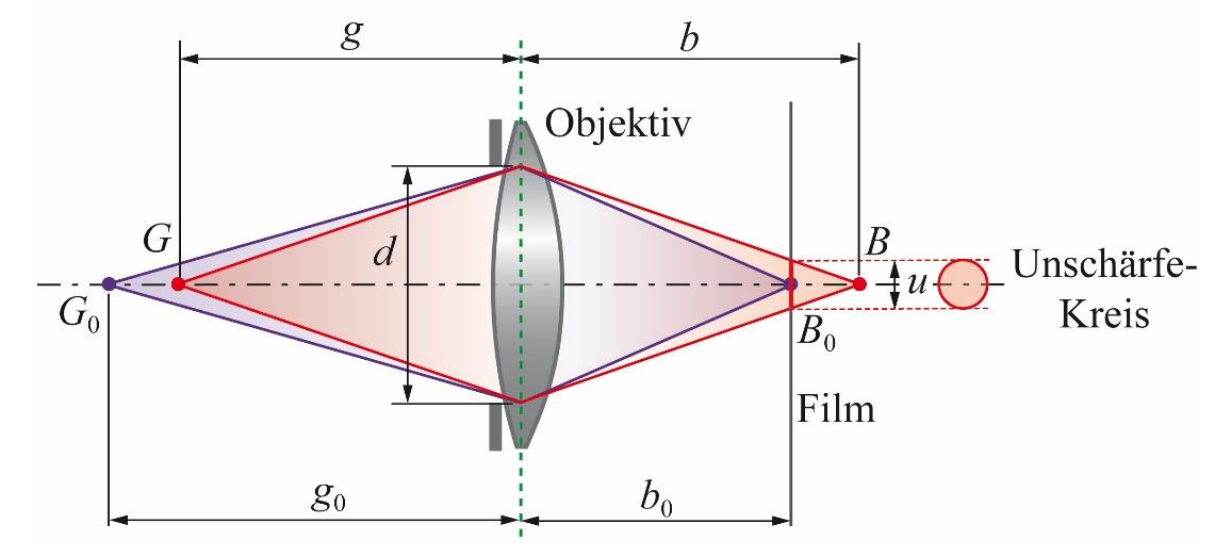
\includegraphics[width=\linewidth]{Bilder/Wellen-Optik/schaerfentiefe}
\end{minipage}
\hfill
\begin{minipage}{0.3\linewidth}
$$\boxed{ \frac{1}{g} = \frac{1}{g_0} \pm \frac{u}{q \, f^2}  } $$
\end{minipage}

% \vfill\null
% \columnbreak


\begin{tabular}{c l c}
	$b$ & Bildweite & $[b] = \m$ \\
	$b_0$ & $\text{Bilddlistanz}_0$ & $[b_0] = \m$ \\
	$B$ & $\text{Bildgrösse}_0$ & $[B] = \m$ \\
	$B_0$ & $\text{Bild}_0$ & $[B_0] = \m$ \\
	$g$ & Gegenstandsweite ($G$ zu Objektiv) & $[g] = \m$ \\
	$g_0$ & $\text{Gegenstandsdistanz}_0$ ($G_0$ zu Objektiv) & $[g_0] = \m$ \\
	$G$ & Gegenstandsgrösse & $[G] = \m$ \\
	$G_0$ & $\text{Gegenstandsgrösse}_0$ & $[G_0] = \m$ \\
	$f$ & Brennweite & $[f] = \m$ \\
	$u$ & Durchmesser Unschärfekreis & $[d] = \m$ \\
	$d$ & Durchmesser Blendenöffnung & $[d] = \m$ \\
	$v$ & Geschw. des zu fotograf. Objekts & $[v] = \frac{m}{s}$
\end{tabular}






\subsection{Abbildungssysteme - Lupe}


\begin{minipage}{0.48\linewidth}
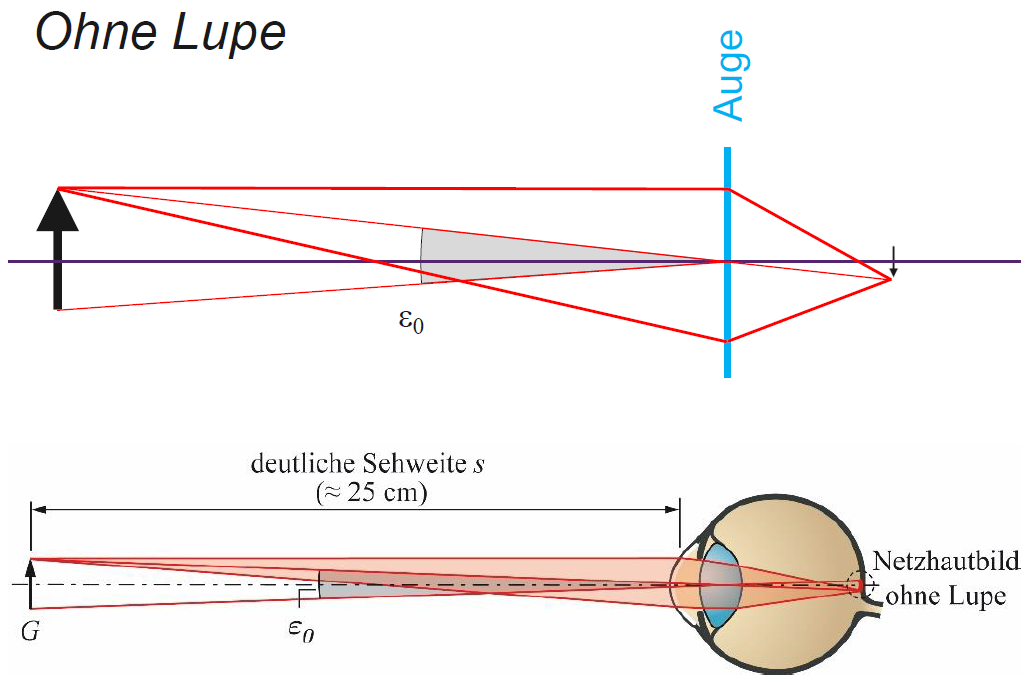
\includegraphics[width=0.9\linewidth]{Bilder/Wellen-Optik/ohne_lupe}

$$ \boxed{ \tan(\varepsilon_0) = \frac{G}{s} } $$
\end{minipage}
\hfill
\begin{minipage}{0.48\linewidth}
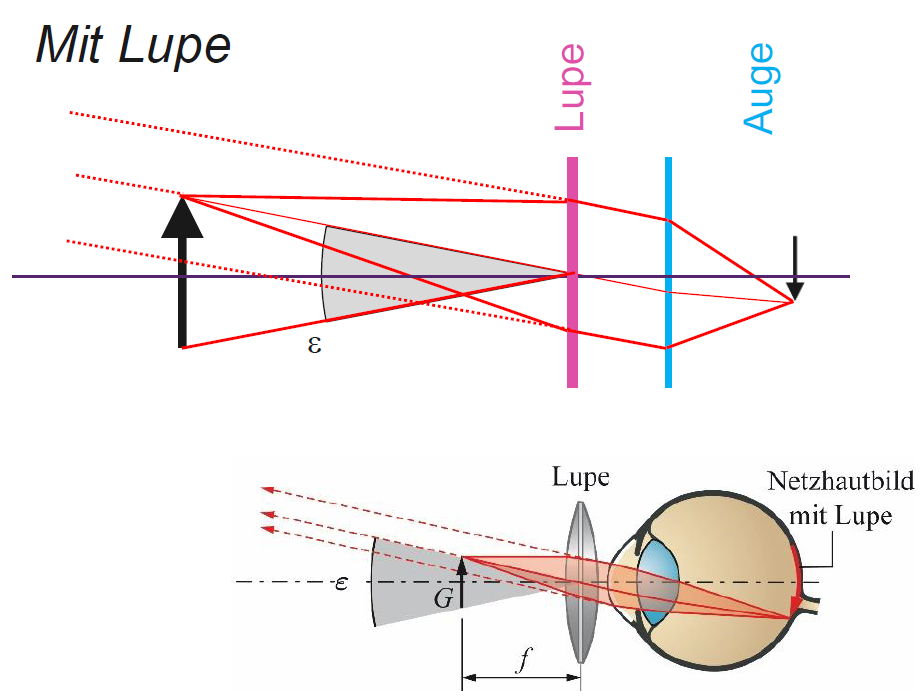
\includegraphics[width=0.9\linewidth]{Bilder/Wellen-Optik/mit_lupe}

$$ \boxed{ \tan(\varepsilon) = \frac{G}{f} } $$
\end{minipage}

$$ \boxed{ V = \frac{\tan(\varepsilon)}{\tan(\varepsilon_0)} = \frac{s}{f} } $$


\begin{tabular}{c l c}
	$\varepsilon_i$ & Sehwinkel & $[\varepsilon_i] =$° \\
	$s$ & Deutliche Sehweite $s =0.25 \, \m$ & $[s] = \m$ \\
	$f$ & Brennweite & $[f] = \m$ \\
	$V$ & Vergrösserung & $[V] = 1$ \\
\end{tabular}


\subsection{Abbildungssysteme - Fernrohr}

Es wird zuerst ein vergrössertes Bild erzeugt, welchs selber wiederum mit einer Lupe betrachtet wird. \\

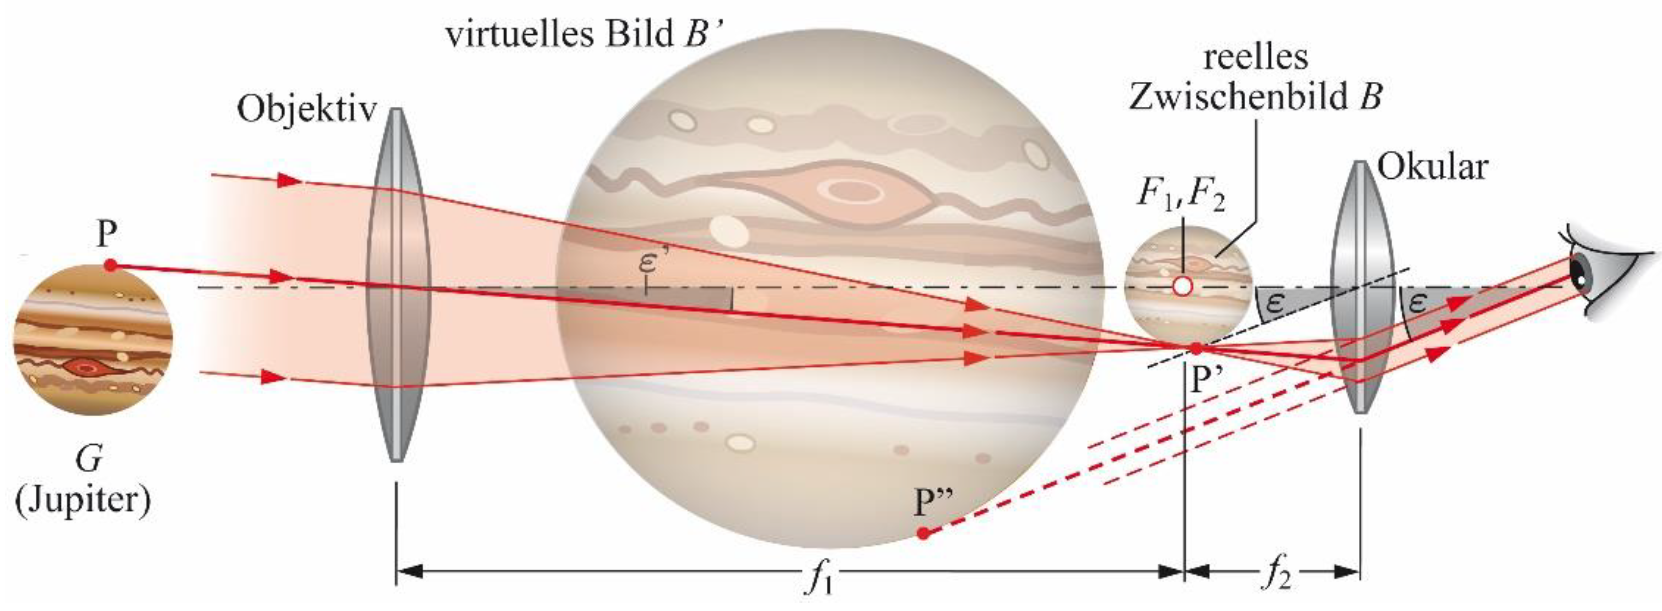
\includegraphics[width=0.9\linewidth]{Bilder/Wellen-Optik/fernrohr} \\

$$ \boxed{ V = \frac{\tan(\varepsilon)}{\tan(\varepsilon')} = \frac{\frac{B}{f_2}}{\frac{B}{f_1} } = \frac{f_1}{f_2}  } $$


% \vfill\null
% \columnbreak


\subsection{Abbildungssysteme - Mikroskop}

Es wird zuerst ein vergrössertes Bild erzeugt, welchs selber wiederum mit einer Lupe betrachtet wird. \\

\includegraphics[width=0.9\linewidth]{Bilder/Wellen-Optik/mikroskop} \\

$$ \boxed{ V = \underbrace{\frac{\Delta}{f_1}}_{V_1} \cdot \underbrace{\frac{s}{f_2}}_{V_2} = \frac{\tan(\varepsilon)}{\tan(\varepsilon_0)} = \frac{\frac{B}{f_2}}{\frac{G}{s}} = \frac{B}{G} \frac{s}{f_2} = \frac{b_1}{g_1} \frac{s}{f_2} } $$


\begin{tabular}{c l c}
	$\varepsilon_i$ & Sehwinkel & $[\varepsilon_i] =$° \\
	$s$ & Deutliche Sehweite $s =0.25 \, \m$ & $[s] = \m$ \\
	$f_i$ & Brennweite & $[f_i] = \m$ \\
	$V$ & Vergrösserung & $[V] = 1$ \\
	$V_1$ & Vergrösserung des Objektivs & $[V_1] = 1$ \\
	$V_2$ & Vergrösserung des Okulars & $[V_2] = 1$ \\
	$\Delta$ & optische Tubuslänge (Abstand der Brennpunkte) & $[\Delta] = \m$ \\
	$b_1$ & Bildweite & $[b_1] = \m$ \\
	$g_1$ & Gegenstandsweite & $[g_1] = \m$ \\
	$B$ & Bildgrösse & $[B] = \m$ \\
	$G$ & Gegenstandsgrösse & $[G] = \m$
\end{tabular}






\subsection{Farbentheorie}

\begin{tabularx}{\linewidth}{lX}
	Spektralfarben: & Die gesamten Lichtfarben \\
	Mischfarben:    & Mischung von versch. Spektralfarben \\
	Grundfarben:    & Ein Set, um alle Mischfarben zu erzeugen \\
	Komplementärfarben: & Mischfarbe, die bleibt, wenn von weissem Licht eine Farbe ausgeblendet wird \\
	Monochromatisches Licht: & Nur eine einzige Wellenlänge (Farbe) 
\end{tabularx}



\subsubsection{Farbmischungen}

\begin{minipage}{0.48\linewidth}
\textbf{Additive Farbmischung} \\

\includegraphics[width=0.9\linewidth]{Bilder/Wellen-Optik/additiveFarbmischung}

\end{minipage}
\hfill
\begin{minipage}{0.48\linewidth}
\textbf{Subtraktive Farbmischung} \\

\includegraphics[width=0.9\linewidth]{Bilder/Wellen-Optik/SubtraktiveFarbmischung}
\end{minipage}